% !TeX encoding = UTF-8
% !TeX TS-program = latexmk
% Mathematical Programming: An Introduction to Optimization
% Faithful reconstruction of source PDF pages 1--80.
% Except for the documented corrections, slide titles, prose, equations,
% examples, ordering, and figure captions reproduce the source deck.
% See mathematical-programming-2026-2027-corrections.md for every change.

\PassOptionsToPackage{cmyk}{xcolor}
\documentclass[aspectratio=169,hyperref,UTF8,CJK]{beamer}

\makeatletter
\newcommand{\beamer@scu@fontextend}{%
  \setsansfont{Latin Modern Sans}%
  \setmonofont{Latin Modern Mono}%
}
\makeatother

\usetheme[
  ColorDisplay=JXred,
  BlockDisplay=followtheme,
  CodeTheme=listing,
  LanguageMode=en,
  Miniframes=follow,
  NavigationTool=1-2-3,
  FontTheme=Custom,
  MathFont=LM,
  BIBMode=none,
  ContentMuticols=false,
  Background=SCU-Full
]{scu}

\usepackage{array}
\usepackage{booktabs}
\usepackage{mathtools}
\usepackage{multirow}
\usepackage{tabularx}
\usepackage{arydshln}

\newcommand{\R}{\mathbb{R}}
\newcommand{\trans}{\mathsf{T}}
\newcommand{\vect}[1]{\boldsymbol{#1}}

\title[Introduction to Optimization]{Introduction to Optimization}
\subtitle{Mathematical Programming}
\author[Changxi Wang]{Changxi Wang}
\institute{Sichuan University-Pittsburgh Institute\\Chengdu, China}
\date{2026--2027 Academic Year}

% Disable the theme's extra subsection-outline pages so source page n remains
% output page n (automatic title page plus 79 content frames).
\AtBeginSubsection[]{}

\begin{document}

% Source PDF page 001: title page. Instructor and academic year updated.

\section{Introduction}
\subsection{Course Information}

% Source PDF page 002
\begin{frame}{About the Course}
  \begin{itemize}
    \item Credit hours: 48
    \item Textbook: \emph{Mathematical Programming: An Introduction to Optimization}, by Melvyn W. Jeter
    \item Reference: \emph{Convex Optimization}, by Stephen Boyd
    \item Performance Assessment:
      \begin{enumerate}
        \item Class attendance (10\%)
        \item Assignments (40\%)
        \item Final Exam (50\%)
      \end{enumerate}
  \end{itemize}
\end{frame}

% Source PDF page 003. The first-person attribution was corrected because the
% acknowledged contributors belong to the source deck's former course team.
\begin{frame}{Acknowledgments}
  \small
  The source lecture notes acknowledge
  % \begin{columns}[T,onlytextwidth]
  %   \begin{column}{0.31\textwidth}
  %     \centering
  %     \includegraphics[width=0.72\linewidth,height=0.25\textheight,keepaspectratio]{figures/mp-2026/p003-yang-yan.jpg}\\[-1mm]
  %     YANG, Yan
  %   \end{column}
  %   \begin{column}{0.31\textwidth}
  %     \centering
  %     
\includegraphics[width=0.72\linewidth,height=0.25\textheight,keepaspectratio]{figures/mp-2026/p003-liao-sijia.jpg}\\[-1mm]
  %     LIAO, Sijia
  %   \end{column}
  %   \begin{column}{0.31\textwidth}
  %     \centering
  %     
\includegraphics[width=0.72\linewidth,height=0.25\textheight,keepaspectratio]{figures/mp-2026/p003-yan-jiajun.jpg}\\[-1mm]
  %     YAN, Jiajun
  %   \end{column}
  % \end{columns}
  % \vspace{1mm}
  % for:
  \begin{itemize}
    \item preparing the lecture notes
    \item acting as teaching assistants
    \item monitoring possible mistakes in the source deck
  \end{itemize}
\end{frame}

% Source PDF page 004
\begin{frame}{Introduction}
  \begin{itemize}
    \item An introduction to optimization for students with background of linear algebra, calculus, and multivariable calculus
    \item Optimization is used everywhere nowadays with growing importance
    \item Applications:
      \begin{itemize}
        \item Economic analysis
        \item Management
        \item Engineering technology
        \item Military operations
        \item etc
      \end{itemize}
  \end{itemize}
\end{frame}

% Source PDF page 005
\begin{frame}{Examples}
  \centering
  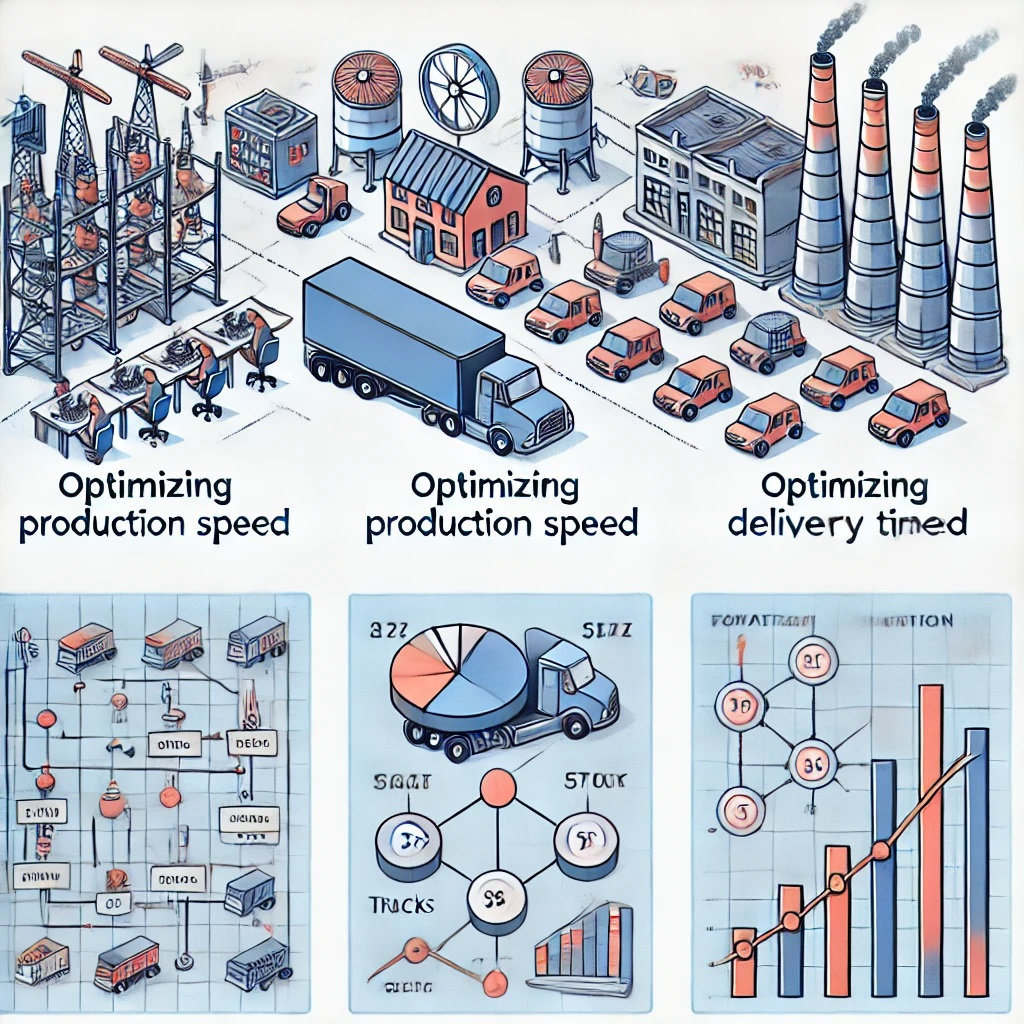
\includegraphics[width=0.77\linewidth,height=0.76\textheight,keepaspectratio]{figures/mp-2026/p005-optimization-manufacturing.jpg}
\end{frame}

% Source PDF page 006
\begin{frame}{Examples}
  \centering
  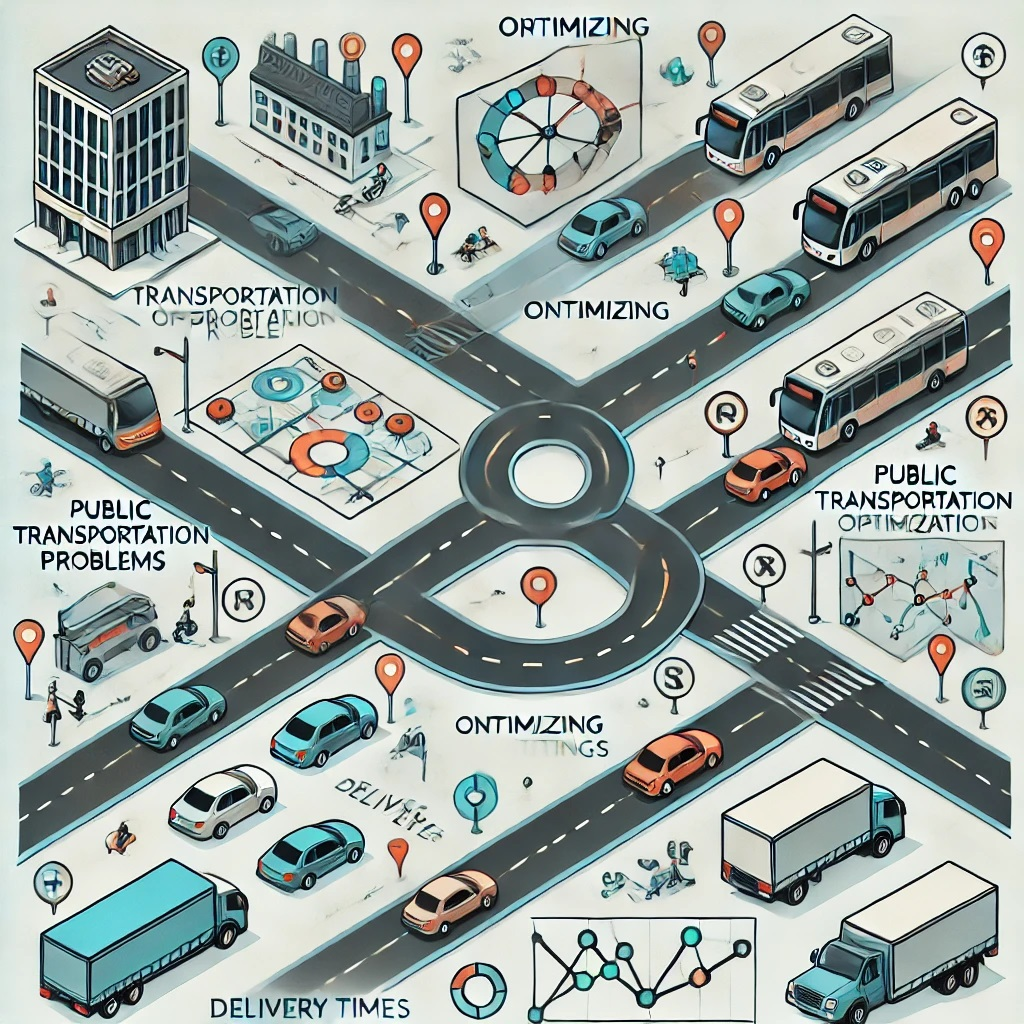
\includegraphics[width=0.77\linewidth,height=0.76\textheight,keepaspectratio]{figures/mp-2026/p006-optimization-transportation.jpg}
\end{frame}

\section{Mathematical Programming Problems}
\subsection{Basic Models}

% Source PDF page 007
\begin{frame}{The Basic Mathematical Programming Problem}
  \small
  \begin{itemize}
    \item Definition:
      \begin{align}
        \min\ f(x_1,x_2,\ldots,x_n)\quad &\text{or}\quad \max\ f(x_1,x_2,\ldots,x_n) \tag{1}\\
        \text{s.t.}\quad &(x_1,x_2,\ldots,x_n)\in\Omega \tag{2}
      \end{align}
      where
      \begin{itemize}
        \item $f(x_1,x_2,\ldots,x_n)$ in (1) is the cost (objective) function.
        \item $\Omega$ in (2) is the set of feasible solutions.
      \end{itemize}
    \item Unconstrained problem: $\Omega=\{(x_1,\ldots,x_n):x_i\in\R\}$.
    \item Constrained problem: $\Omega$ is a proper subset of $\{(x_1,\ldots,x_n):x_i\in\R\}$.
  \end{itemize}
\end{frame}

% Source PDF page 008
\begin{frame}{Linear Programming Problem}
  \footnotesize
  \begin{itemize}
    \item Linear cost function:
      \begin{equation}\tag{3}
        f(x_1,\ldots,x_n)=c_1x_1+\ldots+c_nx_n,
      \end{equation}
      where $c_1,\ldots,c_n$ are real constants. $c_i$ is called the cost coefficient of the variable $x_i$.
    \item An equality constraint:
      \begin{equation}\tag{4}
        a_1x_1+\ldots+a_nx_n=b,
      \end{equation}
      where $a_1,\ldots,a_n$ are real constants.
    \item A linear inequality constraint:
      \begin{equation}\tag{5}
        a_1x_1+\ldots+a_nx_n\gtreqless b,
      \end{equation}
    \item A problem that is NOT linear programming: nonlinear programming problem.
    \item Generally, linear programming problems are easier than nonlinear ones.
  \end{itemize}
\end{frame}

\subsection{Examples}

% Source PDF page 009
\begin{frame}{Example 1}
  \small
  \begin{itemize}
    \item A manufacturer produces $n$ products $P_1,P_2,\ldots,P_n$ from $m$ raw materials $M_1,\ldots,M_m$. The amount of each raw material required for each product:
      \begin{center}
        \begin{tabular}{c|cccc}
          & $P_1$ & $P_2$ & $\cdots$ & $P_n$\\ \hline
          $M_1$ & $a_{1,1}$ & $a_{1,2}$ & $\cdots$ & $a_{1,n}$\\
          $M_2$ & $a_{2,1}$ & $a_{2,2}$ & $\cdots$ & $a_{2,n}$\\
          $\vdots$ & $\vdots$ & $\vdots$ & $\ddots$ & $\vdots$\\
          $M_m$ & $a_{m,1}$ & $a_{m,2}$ & $\cdots$ & $a_{m,n}$
        \end{tabular}
      \end{center}
    \item Available: $b_i$ units of $M_i$, $\forall i=1,\ldots,m$.
    \item Revenue: $c_j$ dollars for each unit of $P_j$ sold.
    \item Question: Desire to maximize the total daily revenue.
  \end{itemize}
\end{frame}

% Source PDF page 010
\begin{frame}{Example 1}
  \begin{itemize}
    \item $x_j$: \# of product $P_j$ that has been produced.
    \item $a_{i,j}x_j$: \# of material $M_i$ used to produce $x_j$ units of $P_j$.
    \item \# of the daily revenue:
      \begin{equation}\tag{6}
        c_1x_1+\ldots+c_nx_n
      \end{equation}
    \item \# of material $M_i$ consumed in total:
      \begin{equation}\tag{7}
        a_{i,1}x_1+\ldots+a_{i,n}x_n\le b_i,
      \end{equation}
  \end{itemize}
\end{frame}

% Source PDF page 011
\begin{frame}{Example 1}
  \small
  \begin{itemize}
    \item The cost function:
      \begin{equation}\tag{8}
        \max_{x_j,\,\forall j\in[1,n]}\{c_1x_1+\ldots+c_nx_n\}
      \end{equation}
      subject to
      \begin{equation}\tag{9}
      \begin{aligned}
        a_{1,1}x_1+a_{1,2}x_2+\ldots+a_{1,n}x_n&\le b_1,\\
        a_{2,1}x_1+a_{2,2}x_2+\ldots+a_{2,n}x_n&\le b_2,\\
        &\vdots\\
        a_{m,1}x_1+a_{m,2}x_2+\ldots+a_{m,n}x_n&\le b_m,\\
        x_1\ge0,\ x_2\ge0,\ldots,\ x_n&\ge0.
      \end{aligned}
      \end{equation}
  \end{itemize}
\end{frame}

% Source PDF page 012
\begin{frame}{Example 1}
  \small
  \begin{itemize}
    \item Continuous variable: allowed to take on all fractional as well as integral values within its range of variation
    \item Discrete variable: must take on values from a discrete set of values
    \item Slack variable: inequality can be converted to an equality constraint by adding a non-negative variable
      \begin{itemize}
        \item Take (9) for example:
          \begin{equation*}
            a_{1,1}x_1+\ldots+a_{1,n}x_n+x_{n+1}=b_1,
          \end{equation*}
          $x_{n+1}$: Slack variable, assigned a cost coefficient of $c_{n+1}=0$
      \end{itemize}
  \end{itemize}
\end{frame}

% Source PDF page 013
\begin{frame}{Example 1}
  \footnotesize
  \begin{itemize}
    \item The cost function (8) can be reformulated as
      \begin{equation*}
        \max_{x_j,\,\forall j\in[1,n+m]}
        \underbrace{\{c_1x_1+\ldots+c_nx_n+c_{n+1}x_{n+1}+\ldots+c_{n+m}x_{n+m}\}}
        _{=\max_{x_j,\,\forall j\in[1,n]}\{c_1x_1+\ldots+c_nx_n\}}
      \end{equation*}
      subject to
      \begin{align*}
        a_{1,1}x_1+a_{1,2}x_2+\ldots+a_{1,n}x_n+x_{n+1}&=b_1,\\
        a_{2,1}x_1+a_{2,2}x_2+\ldots+a_{2,n}x_n+x_{n+2}&=b_2,\\
        &\vdots\\
        a_{m,1}x_1+a_{m,2}x_2+\ldots+a_{m,n}x_n+x_{n+m}&=b_m,\\
        x_1\ge0,\ldots,x_n\ge0,\quad x_{n+1}\ge0,\ldots,x_{n+m}&\ge0.
      \end{align*}
  \end{itemize}
\end{frame}

% Source PDF page 014
\begin{frame}{Example 2}
  \begin{itemize}
    \item 4 salesmen + 4 sales districts
    \item The sales productivity ratings for each salesman $S_i$ in each sales districts $D_j$:
      \begin{center}
        \begin{tabular}{c|rrrr}
          & $D_1$ & $D_2$ & $D_3$ & $D_4$\\ \hline
          $S_1$ & 5 & 10 & 8 & 2\\
          $S_2$ & 3 & 4 & 2 & 6\\
          $S_3$ & 9 & 5 & 4 & 5\\
          $S_4$ & 5 & 5 & 6 & 4
        \end{tabular}
      \end{center}
    \item Question: Determine the best assignment of salesman to sales districts.
  \end{itemize}
\end{frame}

% Source PDF page 015
\begin{frame}{Example 2}
  \footnotesize
  \begin{itemize}
    \item Define
      \begin{equation}\tag{10}
        x_{i,j}=\begin{cases}1,&\text{if $S_i$ assigned to $D_j$},\\0,&\text{otherwise.}\end{cases}
      \end{equation}
    \item The value of an assignment:
      \begin{align*}
        f(x_{i,j})={}&5x_{1,1}+10x_{1,2}+8x_{1,3}+2x_{1,4}+3x_{2,1}+4x_{2,2}+2x_{2,3}+6x_{2,4}\\
        &+9x_{3,1}+5x_{3,2}+4x_{3,3}+5x_{3,4}+5x_{4,1}+5x_{4,2}+6x_{4,3}+4x_{4,4}.
      \end{align*}
    \item Each salesman must be assigned to exactly one district:
      \begin{equation}\tag{11}
        \sum_{j=1}^{4}x_{i,j}=1,\qquad \forall i.
      \end{equation}
    \item Each district is assigned exactly one salesman:
      \begin{equation}\tag{12}
        \sum_{i=1}^{4}x_{i,j}=1,\qquad \forall j.
      \end{equation}
  \end{itemize}
\end{frame}

% Source PDF page 016
\begin{frame}{Example 2}
  \begin{itemize}
    \item Problem:
      \begin{equation*}
        \max_{\forall i,j}\{f(x_{i,j})\}
      \end{equation*}
      subject to
      \begin{align*}
        x_{i,1}+x_{i,2}+x_{i,3}+x_{i,4}&=1, &&\forall i,\\
        x_{1,j}+x_{2,j}+x_{3,j}+x_{4,j}&=1, &&\forall j,\\
        0\le x_{i,j}&\le1, &&\forall i,j.
      \end{align*}
  \end{itemize}
\end{frame}

% Source PDF page 017
\begin{frame}{Example 3}
  \small
  \begin{itemize}
    \item A flour company has 3 production lines which can produce A and B. The number of ten pound sacks of flour which can be produced daily by each of the production lines is summarized in the following table:
      \begin{center}
        \begin{tabular}{c|rrr}
          & $L_1$ & $L_2$ & $L_3$\\ \hline
          A & 15000 & 10000 & 12000\\
          B & 12000 & 13500 & 14500
        \end{tabular}
      \end{center}
    \item Question: Produce as many ten pound bags of flour of brands A and B as possible.
  \end{itemize}
\end{frame}

% Source PDF page 018
\begin{frame}{Example 3}
  \small
  \begin{itemize}
    \item Define
      \begin{equation*}
        x_i=\begin{cases}1,&\text{if $L_i$ assigned to A},\\0,&\text{otherwise,}\end{cases}
        \qquad
        w_i=\begin{cases}1,&\text{if $L_i$ assigned to B},\\0,&\text{otherwise.}\end{cases}
      \end{equation*}
    \item A production line cannot be assigned to both products:
      \begin{equation*}
        x_1w_1=0,\quad x_2w_2=0,\quad x_3w_3=0.
      \end{equation*}
    \item All variables are non-negative
  \end{itemize}
\end{frame}

% Source PDF page 019
\begin{frame}{Example 3}
  \begin{itemize}
    \item The above two constraints can be compressed into one:
      \begin{equation}\tag{13}
        \sum_{i=1}^{3}x_iw_i=x_1w_1+x_2w_2+x_3w_3=0.
      \end{equation}
    \item To insure that each production line is assigned to a job:
      \begin{align*}
        x_1+w_1&=1,\\
        x_2+w_2&=1,\\
        x_3+w_3&=1.
      \end{align*}
  \end{itemize}
\end{frame}

% Source PDF page 020
\begin{frame}{Example 3}
  \small
  \begin{itemize}
    \item A nonlinear programming problem:
      \begin{equation*}
        \max_{\forall x_i,w_j}\{15000x_1+10000x_2+12000x_3+12000w_1+13500w_2+14500w_3\}
      \end{equation*}
      subject to
      \begin{align*}
        x_1+w_1&=1,\\
        x_2+w_2&=1,\\
        x_3+w_3&=1,\\
        \sum_{i=1}^{3}x_iw_i&=0,\quad\text{(complementary constraint)}\\
        0\le x_i\le1,\quad 0\le w_i&\le1,\quad\forall i.
      \end{align*}
  \end{itemize}
\end{frame}

% Source PDF page 021
\begin{frame}{Example 4}
  \small
  \begin{itemize}
    \item Quadratic (nonlinear) programming problem:
      \begin{equation*}
        \max_{\forall i,j}\left\{c_1x_1+\ldots+c_nx_n+\sum_{i=1}^{n}\sum_{j=1}^{n}b_{ij}x_ix_j\right\}
      \end{equation*}
      subject to
      \begin{align*}
        a_{11}x_1+a_{12}x_2+\ldots+a_{1n}x_n&=b_1,\\
        a_{21}x_1+a_{22}x_2+\ldots+a_{2n}x_n&=b_2,\\
        &\vdots\\
        a_{m1}x_1+a_{m2}x_2+\ldots+a_{mn}x_n&=b_m,\\
        x_1\ge0,\quad x_2\ge0,\ldots,\quad x_n&\ge0.
      \end{align*}
  \end{itemize}
\end{frame}

% Source PDF page 022
\begin{frame}{Example 4}
  \small
  \begin{itemize}
    \item The portfolio selection problem:
      \begin{equation*}
        \max_{\forall i,j}\left\{c_1x_1+\ldots+c_nx_n-\sum_{i=1}^{n}\sum_{j=1}^{n}b_{i,j}x_ix_j\right\}
      \end{equation*}
      subject to
      \begin{align*}
        x_1+\ldots+x_n&=1,\\
        x_1\ge0,\ldots,x_n&\ge0.
      \end{align*}
    \item $x_i$: investment
    \item $c_i$: expected rate of return
    \item $\sum_{i=1}^{n}\sum_{j=1}^{n}b_{i,j}x_ix_j$: risk of investment
  \end{itemize}
\end{frame}

\subsection{Solutions, Topology, and Sensitivity}

% Source PDF page 023
\begin{frame}{Global And Local Solutions}
  \begin{itemize}
    \item Standard Euclidean distance:
      \begin{equation*}
        \lVert\vect{x}-\bar{\vect{x}}\rVert=\sqrt{\sum_{i=1}^{n}(x_i-\bar{x}_i)^2}
      \end{equation*}
    \item Neighborhood of $\bar{\vect{x}}$:
      \begin{equation*}
        N_{\varepsilon}(\bar{\vect{x}})=\{\vect{x}:\lVert\vect{x}-\bar{\vect{x}}\rVert<\varepsilon\}
      \end{equation*}
      where $\varepsilon$ is a positive real number.
  \end{itemize}
\end{frame}

% Source PDF page 024. Strict-minimum comparison point corrected; irrelevant
% existential epsilon removed from the two global definitions.
\begin{frame}{Global And Local Solutions}
  \small
  \begin{itemize}
    \item Local minimum (at $\bar{\vect{x}}\in\Omega$):
      \begin{equation*}
        \exists\varepsilon>0,\ \text{such that }f(\bar{\vect{x}})\le f(\vect{x}),\quad
        \forall\vect{x}\in\Omega\cap N_{\varepsilon}(\bar{\vect{x}}).
      \end{equation*}
    \item Strict local minimum:
      \begin{equation*}
        \exists\varepsilon>0,\ \text{such that }f(\bar{\vect{x}})<f(\vect{x}),\quad
        \forall\vect{x}\in(\Omega\cap N_{\varepsilon}(\bar{\vect{x}}))\setminus\{\bar{\vect{x}}\}.
      \end{equation*}
    \item Global minimum:
      \begin{equation*}
         \exists\varepsilon>0,\ \text{such that }f(\bar{\vect{x}})\le f(\vect{x}),\quad\forall\vect{x}\in\Omega.
      \end{equation*}
    \item Strict global minimum:
      \begin{equation*}
         \exists\varepsilon>0,\ \text{such that }f(\bar{\vect{x}})<f(\vect{x}),\quad\forall\vect{x}\in\Omega\setminus\{\bar{\vect{x}}\}.
      \end{equation*}
  \end{itemize}
\end{frame}

% Source PDF page 025
\begin{frame}{Topology Concepts}
  \small
  \begin{itemize}
    \item The interior of $\Omega$:
      \begin{equation*}
        \operatorname{Int}(\Omega)=\{\vect{x}\in\Omega:N_{\varepsilon}(\vect{x})\subseteq\Omega\text{ for some }\varepsilon>0\}.
      \end{equation*}
    \item $\Omega$ is open if $\Omega=\operatorname{Int}(\Omega)$, i.e., every point of $\Omega$ is an interior point
    \item The exterior of $\Omega$:
      \begin{equation*}
        \operatorname{Ext}(\Omega)=\{\vect{x}:N_{\varepsilon}(\vect{x})\subseteq E^n\setminus\Omega\text{ for some }\varepsilon>0\}
      \end{equation*}
      where
      \begin{align*}
        E^n&=\{\vect{x}=(x_1,\ldots,x_n):x_i\in\R\},\\
        E^n\setminus\Omega&=\{\vect{x}\in E^n:\vect{x}\notin\Omega\}.
      \end{align*}
  \end{itemize}
\end{frame}

% Source PDF page 026
\begin{frame}{Topology Concepts}
  \small
  \begin{itemize}
    \item $\vect{x}$ is a boundary point of $\Omega$:
      \begin{align*}
        \exists\vect{x}_1\in\Omega:&\quad\vect{x}_1\in N_{\varepsilon}(\vect{x}),\quad\forall\varepsilon>0,\\
        \exists\vect{x}_2\notin\Omega:&\quad\vect{x}_2\in N_{\varepsilon}(\vect{x}),\quad\forall\varepsilon>0.
      \end{align*}
    \item The boundary $\operatorname{Bd}(\Omega)$:
      \begin{equation*}
        \text{The collection of all boundary points of }\Omega
      \end{equation*}
    \item A set $\Omega$ is closed:
      \begin{equation*}
        \operatorname{Bd}(\Omega)\subseteq\Omega
      \end{equation*}
    \item $\vect{x}$ is an accumulation point of $\Omega$:
      \begin{equation*}
        \exists\vect{x}'\ne\vect{x},\quad \vect{x}'\in\Omega:\quad
        \vect{x}'\in N_{\varepsilon}(\vect{x}),\quad\forall\varepsilon>0.
      \end{equation*}
  \end{itemize}
\end{frame}

% Source PDF page 027. Source typo ``Post-otimal'' corrected.
\begin{frame}{Post-Optimal (Sensitivity) Analysis}
  \begin{itemize}
    \item Data in a mathematical programming problem can change as conditions change: Data $\rightarrow$ Estimates/Measurements
    \item Possible to solve new problem by modifying the original one, thus avoiding completely solving the new problem
    \item Post-optimal analysis:
      \begin{equation*}
        \begin{array}{c}\text{optimal solution of}\\[-1mm]\text{existing problem}\end{array}
        \quad\longrightarrow\quad
        \begin{array}{c}\text{optimal solution of}\\[-1mm]\text{modified problem}\end{array}
      \end{equation*}
  \end{itemize}
\end{frame}

% Source PDF page 028
\begin{frame}{Example 5}
  \begin{itemize}
    \item A company's products are stored in $m$ places, and sold in $n$ outlets
    \item Shipping cost from the $i$-th storage to the $j$-th outlet: $c_{i,j}$ dollars
    \item One day, each outlet requires exactly $d_j$ units of product
    \item Each storage has $s_i$ units of product available for shipment
    \item Question: To minimize the shipping cost, determine the number of units should be shipped from each storage to each outlet
  \end{itemize}
\end{frame}

% Source PDF page 029
\begin{frame}{Example 5}
  \small
  \begin{itemize}
    \item Question: To minimize the shipping cost, determine the number of units should be shipped from each storage to each outlet
      \begin{equation*}
        \min_{x_{i,j}}\sum_{i=1}^{m}\sum_{j=1}^{n}c_{i,j}x_{i,j}
      \end{equation*}
      subject to
      \begin{align*}
        \sum_{j=1}^{n}x_{i,j}&\le s_i, &&\forall i,\\
        \sum_{i=1}^{m}x_{i,j}&=d_j, &&\forall j,\\
        x_{i,j}&\ge0, &&\forall i,j.
      \end{align*}
  \end{itemize}
\end{frame}

% Source PDF page 030
\begin{frame}{Parametric Programming Problem}
  \small
  \begin{itemize}
    \item Question: Product is good. Customers want more. Outlet requires an increase of $\bar d_j$ per day, and after $t$ days
      \begin{equation*}
        \min_{x_{i,j}}\sum_{i=1}^{m}\sum_{j=1}^{n}c_{i,j}x_{i,j}
      \end{equation*}
      subject to
      \begin{align*}
        \sum_{j=1}^{n}x_{i,j}&\le s_i, &&\forall i,\\
        \sum_{i=1}^{m}x_{i,j}&=d_j+t\bar d_j, &&\forall j,\\
        x_{i,j}&\ge0, &&\forall i,j,\\
        t&\ge0.
      \end{align*}
  \end{itemize}
\end{frame}

% Source PDF page 031
\begin{frame}{Model Stability}
  \footnotesize
  \begin{itemize}
    \item \textcolor{blue}{Model Stable}: small changes in the data $\rightarrow$ small changes in $x_1^*,\ldots,x_n^*$ and $f(x_1^*,\ldots,x_n^*)$
    \item \textcolor{red}{Model Unstable}: small changes in the data $\rightarrow$ LARGE changes in $x_1^*,\ldots,x_n^*$ and $f(x_1^*,\ldots,x_n^*)$
    \item Frequently, model-unstable problems possess redundant constraints
      \begin{columns}[T,onlytextwidth]
        \begin{column}{0.47\textwidth}
          \begin{align*}
            g_i(x_1,\ldots,x_n)&=b_i,\quad\forall i,\\
            \sum_{i=1}^{m}\lambda_i g_i(x_1,\ldots,x_n)&=\sum_{i=1}^{m}\lambda_i b_i
          \end{align*}
          \centering Feasible problem
        \end{column}
        \begin{column}{0.04\textwidth}
          \centering\vspace{8mm}$\Rightarrow$
        \end{column}
        \begin{column}{0.47\textwidth}
          \begin{align*}
            g_i(x_1,\ldots,x_n)&=b_i,\quad\forall i,\\
            \sum_{i=1}^{m}\lambda_i g_i(x_1,\ldots,x_n)&=\varepsilon+\sum_{i=1}^{m}\lambda_i b_i
          \end{align*}
          \centering Infeasible problem
        \end{column}
      \end{columns}
  \end{itemize}
\end{frame}

\section{A Review of Linear Algebra}
\subsection{Matrices and Vectors}

% Source PDF page 032
\begin{frame}{A Review of Linear Algebra: Matrix}
  \begin{itemize}
    \item Matrix:
      \begin{equation*}
        A=\begin{bmatrix}
          a_{1,1}&a_{1,2}&\cdots&a_{1,n}\\
          a_{2,1}&a_{2,2}&\cdots&a_{2,n}\\
          \vdots&\vdots&\ddots&\vdots\\
          a_{m,1}&a_{m,2}&\cdots&a_{m,n}
        \end{bmatrix}
      \end{equation*}
    \item Compact expression: $A=[a_{i,j}]$
      \begin{itemize}
        \item $a_{i,j}$: the $(i,j)$-th entry of $A$
        \item $\R^{m\times n}$: The collection of all $m\times n$ real matrices
      \end{itemize}
  \end{itemize}
\end{frame}

% Source PDF page 033
\begin{frame}{A Review of Linear Algebra: Matrix}
  \begin{itemize}
    \item The transpose of $A$:
      \begin{equation*}
        A^{\trans}=\begin{bmatrix}
          a_{1,1}&a_{2,1}&\cdots&a_{m,1}\\
          a_{1,2}&a_{2,2}&\cdots&a_{m,2}\\
          \vdots&\vdots&\ddots&\vdots\\
          a_{1,n}&a_{2,n}&\cdots&a_{m,n}
        \end{bmatrix}
      \end{equation*}
  \end{itemize}
\end{frame}

% Source PDF page 034
\begin{frame}{A Review of Linear Algebra: Vector}
  \begin{itemize}
    \item Column matrix (vector):
      \begin{equation*}
        \vect{x}=\begin{bmatrix}x_1\\\vdots\\x_m\end{bmatrix}
        =[x_1,\ldots,x_m]^{\trans}\in\R^{m\times1}
      \end{equation*}
    \item Row matrix:
      \begin{equation*}
        \vect{y}^{\trans}=[y_1,\ldots,y_n]\in\R^{1\times n}
      \end{equation*}
    \item \textcolor{blue}{Scalars}: real/complex numbers
    \item \textcolor{blue}{Vector space} ($\R^{m\times1}$): Euclidean $m$-space ($E^m$)
  \end{itemize}
\end{frame}

% Source PDF page 035
\begin{frame}{A Review of Linear Algebra: Vector}
  \begin{itemize}
    \item Vector addition:
      \begin{equation*}
        \vect{x}+\vect{y}=[x_1+y_1,\ldots,x_n+y_n]^{\trans},qquad
        \vect{x},\vect{y}\in\R^{n\times1}
      \end{equation*}
    \item For a scalar $\alpha$, scalar multiplication:
      \begin{equation*}
        \alpha\vect{x}=[\alpha x_1,\ldots,\alpha x_n]^{\trans}
      \end{equation*}
  \end{itemize}
\end{frame}

% Source PDF page 036. The free index in the source inner product and the
% incorrect vector in the norm were corrected.
\begin{frame}{A Review of Linear Algebra: Vector}
  \begin{itemize}
    \item Inner product:
      \begin{equation*}
        \vect{x}^{\trans}\vect{y}=\langle\vect{x},\vect{y}\rangle
        =\sum_{i=1}^{n}x_i y_i
      \end{equation*}
    \item Properties:
      \begin{itemize}
        \item $\langle\vect{x},\vect{y}\rangle=\langle\vect{y},\vect{x}\rangle$
        \item $\langle(\alpha\vect{x}+\beta\vect{y}),\vect{z}\rangle
          =\alpha\langle\vect{x},\vect{z}\rangle+\beta\langle\vect{y},\vect{z}\rangle$
        \item $\langle\vect{x},\vect{x}\rangle\ge0$, with equality holds only when $x_i=0$, $\forall i$
        \item Euclidean norm: $\lVert\vect{x}\rVert=\sqrt{\langle\vect{x},\vect{x}\rangle}=\sqrt{\vect{x}^{\trans}\vect{x}}$
      \end{itemize}
  \end{itemize}
\end{frame}

\subsection{Subspaces, Span, and Rank}

% Source PDF page 037
\begin{frame}{A Review of Linear Algebra: Subspace}
  \footnotesize
  \begin{itemize}
    \item \textcolor{red}{Subspace} $S$ of $\R^{n\times1}$: Any \textcolor{blue}{non}empty set of vectors, such that $\vect{x},\vect{y}\in S$, $\alpha,\beta\in\R$, and $\alpha\vect{x}+\beta\vect{y}\in S$
    \item Linear combination:
      \begin{align*}
        \sum_{i=1}^{k}\alpha_i\vect{x}_i
        &=\alpha_1\vect{x}_1+\ldots+\alpha_k\vect{x}_k\\
        &=\left[\sum_{i=1}^{k}\alpha_i x_{i,1},\ldots,
          \sum_{i=1}^{k}\alpha_i x_{i,n}\right]^{\trans}
      \end{align*}
    \item If $B\subseteq\R^{n\times1}$, all linear combination of elements of $B$:
      \begin{equation*}
        L(B)\triangleq\left\{\sum_{i=1}^{k}\alpha_i\vect{x}_i
        \mid \alpha_i\in\R,\ \vect{x}_i\in B,\ k\in\mathbb{N}\right\}
      \end{equation*}
  \end{itemize}
\end{frame}

% Source PDF page 038
\begin{frame}{Example 5}
  \small
  Let $B_1=\{[1,0,0]^{\trans},[0,1,0]^{\trans},[0,0,1]^{\trans}\}$.
  \begin{align*}
    L(B_1)
    &=\{x_1[1,0,0]^{\trans}+x_2[0,1,0]^{\trans}+x_3[0,0,1]^{\trans}:x_1,x_2,x_3\in\R\}\\
    &=\{[x_1,x_2,x_3]^{\trans}:x_1,x_2,x_3\in\R\}\\
    &=\R^{3\times1}.
  \end{align*}
\end{frame}

% Source PDF page 039
\begin{frame}{Example 6}
  \small
  Let $B_2=\{[1,0,0]^{\trans},[1,0,1]^{\trans}\}$.
  \begin{align*}
    L(B_2)
    &=\{x_1[1,0,0]^{\trans}+x_2[1,0,1]^{\trans}:x_1,x_2\in\R\}\\
    &=\{[x_1+x_2,0,x_2]^{\trans}:x_1,x_2\in\R\}.
  \end{align*}
  $L(B_2)$ is the $x_1$-$x_3$ plane.
\end{frame}

% Source PDF page 040
\begin{frame}{Example 6}
  \small
  Let $B_3=\{[1,0,0]^{\trans},[1,0,1]^{\trans},[4,0,1]^{\trans}\}$.
  \begin{align*}
    L(B_3)
    &=\{x_1[1,0,0]^{\trans}+x_2[1,0,1]^{\trans}+x_3[4,0,1]^{\trans}:x_1,x_2,x_3\in\R\}\\
    &=\{[x_1+x_2+4x_3,0,x_2+x_3]^{\trans}:x_1,x_2,x_3\in\R\}.
  \end{align*}
  $L(B_3)=L(B_2)$, i.e., the $x_1$-$x_3$ plane, again.
\end{frame}

% Source PDF page 041
\begin{frame}{A Review of Linear Algebra: Subspace}
  \begin{itemize}
    \item $L(B)$ is a subspace of $\R^{n\times1}$: $L(B)$ is a subspace spanned (or generated) by $B$
    \item If $S=L(B)$, then $B$ spans $S$
    \item[$\diamond$] Any intersection of subspaces of $\R^{n\times1}$ is also a subspace of $\R^{n\times1}$
    \item[$\diamond$] $L(B)$ is the intersection of all subspaces of $\R^{n\times1}$ that contain $B$
      $\longrightarrow$ \textcolor{red}{$L(B)$ is the ``smallest'' subspace that contains $B$}
  \end{itemize}
\end{frame}

% Source PDF page 042
\begin{frame}{Example 7}
  \footnotesize
  Let $S=\{[x_1,x_2,x_3]^{\trans}:x_1+x_2=0,\ x_1,x_2,x_3\in\R\}$.

  \medskip
  Question: Prove that $S$ is a subspace of $\R^{3\times1}$, and find a set that spans $S$

  \medskip
  Solution:
  \begin{align*}
    S&=\{[x_1,x_2,x_3]^{\trans}:x_1+x_2=0,\ x_1,x_2,x_3\in\R\}\\
     &=\{[x_1,-x_1,x_3]^{\trans}:x_1,x_3\in\R\}\\
     &=\{x_1[1,-1,0]^{\trans}+x_3[0,0,1]^{\trans}:x_1,x_3\in\R\}\\
     &=L(\{[1,-1,0]^{\trans},[0,0,1]^{\trans}\}).
  \end{align*}
  $S$ is a subspace that is spanned by $\{[1,-1,0]^{\trans},[0,0,1]^{\trans}\}$.
\end{frame}

% Source PDF page 043. The source used n both for the ambient dimension and
% for the number of selected vectors; this was corrected to k.
\begin{frame}{A Review of Linear Algebra: Subspace}
  \small
  \begin{itemize}
    \item Definition:

      $B\subseteq\R^{n\times1}$, $B$ is a \textcolor{blue}{linearly dependent} set of vectors
      \begin{equation*}
        \Longleftrightarrow
      \end{equation*}
      $\exists$ distinct $\vect{x}_1,\ldots,\vect{x}_k\in B$, $\alpha_1,\ldots,\alpha_k\in\R$, not ALL $\alpha_i=0$, such that
      \begin{equation*}
        \alpha_1\vect{x}_1+\ldots+\alpha_k\vect{x}_k=\vect{0}.
      \end{equation*}
      $\vect{0}$ is the vector having all zero entries, i.e., $\vect{0}=[0,\ldots,0]^{\trans}$
    \item $B$ is a \textcolor{blue}{basis} for $S$ if:
      \begin{enumerate}
        \item $L(B)=S$, i.e., $B$ spans $S$
        \item $B$ is linearly independent
      \end{enumerate}
  \end{itemize}
\end{frame}

% Source PDF page 044
\begin{frame}{A Review of Linear Algebra: Subspace}
  \small
  \begin{itemize}
    \item Theorem 1: Every subspace, $S$ of $\R^{n\times1}$, has a basis. Any two bases of a subspace must contain the same number of elements (\textcolor{blue}{Dimension}).
    \item Theorem 2: Every set of vectors that spans a subspace contains a basis for the subspace.
    \item Theorem 3: Any linearly independent subset of a subspace can be extended to a basis for the space.
    \item Theorem 4: If $S$ is a subspace of $\R^{n\times1}$ with $\dim(S)=k$, then any subset of $S$ that contains more than $k$ vectors is a linearly dependent set of vectors.
      \begin{itemize}
        \item If $S$ and $T$ are both subspace of $\R^{n\times1}$, and $S\subseteq T$, then $\dim(S)\le\dim(T)$.
      \end{itemize}
  \end{itemize}
\end{frame}

% Source PDF page 045
\begin{frame}{A Review of Linear Algebra: Subspace}
  \small
  \begin{itemize}
    \item An $m\times n$ real matrix $A$:
      \begin{equation*}
        A=[a_{i,j}]=\begin{bmatrix}
          a_{1,1}&\cdots&a_{1,j}&\cdots&a_{1,n}\\
          \vdots&\ddots&\vdots&&\vdots\\
          a_{i,1}&\cdots&a_{i,j}&\cdots&a_{i,n}\\
          \vdots&&\vdots&\ddots&\vdots\\
          a_{m,1}&\cdots&a_{m,j}&\cdots&a_{m,n}
        \end{bmatrix}
      \end{equation*}
    \item The $j$-th column of $A$: $A^{(j)}=[a_{1,j},\ldots,a_{i,j},\ldots,a_{m,j}]^{\trans}$
    \item The $i$-th row of $A$: $A_{(i)}=[a_{i,1},\ldots,a_{i,j},\ldots,a_{i,n}]$
  \end{itemize}
\end{frame}

% Source PDF page 046
\begin{frame}{A Review of Linear Algebra: Subspace}
  \begin{itemize}
    \item \textcolor{blue}{Column space}: The space spanned by the columns of $A$, which is a subspace of $\R^{m\times1}$
    \item \textcolor{blue}{Row space}: The space spanned by the rows of $A$, which is a subspace of $\R^{n\times1}$
    \item \textcolor{blue}{Rank}: The dimension of the column (row) space of $A$ is called the column (row) rank of $A$:
      \begin{equation*}
        \operatorname{rank}(A)=\operatorname{rank}_{\mathrm{col}}(A)
        =\operatorname{rank}_{\mathrm{row}}(A)
      \end{equation*}
  \end{itemize}
\end{frame}

\subsection{Matrix Operations and Linear Systems}

% Source PDF page 047
\begin{frame}{A Review of Linear Algebra: Matrix Operation}
  \begin{itemize}
    \item Matrix addition:
      \begin{equation*}A+B=[a_{i,j}+b_{i,j}]\end{equation*}
    \item Matrix scaling:
      \begin{equation*}\alpha A=[\alpha a_{i,j}]\end{equation*}
    \item Matrix product: $A=[a_{i,j}]\in\R^{m\times k}$, $B=[b_{i,j}]\in\R^{k\times n}$
      \begin{equation*}
        AB=\left[\sum_{l=1}^{k}a_{il}b_{lj}\right]\in\R^{m\times n}
      \end{equation*}
  \end{itemize}
\end{frame}

% Source PDF page 048. ``Dirac Function'' corrected to Kronecker delta.
\begin{frame}{A Review of Linear Algebra: Identity Matrix}
  \begin{itemize}
    \item Identity Matrix:
      \begin{equation*}
        I_n=\begin{bmatrix}
          1&0&\cdots&0\\
          0&1&\cdots&0\\
          \vdots&\vdots&\ddots&\vdots\\
          0&0&\cdots&1
        \end{bmatrix}=[\delta_{i,j}]\in\R^{n\times n}
      \end{equation*}
    \item Kronecker delta:
      \begin{equation*}
        \delta_{i,j}=\begin{cases}1,&i=j,\\0,&i\ne j.\end{cases}
      \end{equation*}
  \end{itemize}
\end{frame}

% Source PDF page 049
\begin{frame}{A Review of Linear Algebra: Submatrix}
  \begin{itemize}
    \item $B$ is a submatrix of $A$:
      \begin{equation*}
        A=\begin{bmatrix}
          6&1&3&4&0&5\\
          2&1&4&0&0&1\\
          1&0&1&-1&1&0
        \end{bmatrix},
        \qquad
        B=\begin{bmatrix}4&0&1\\1&-1&0\end{bmatrix}.
      \end{equation*}
  \end{itemize}
\end{frame}

% Source PDF page 050
\begin{frame}{A Review of Linear Algebra: Blocks}
  \small
  \begin{itemize}
    \item Blocks: The submatrices in a partitioned matrix
      \begin{equation*}
        A=\begin{bmatrix}
          6&1&3&4&0&5\\
          2&1&4&0&0&1\\
          1&0&1&-1&1&0
        \end{bmatrix}
        =\begin{bmatrix}B&D&O&\vect{b}\\-\vect{c}_B^{\trans}&-\vect{c}_D^{\trans}&1&0\end{bmatrix},
      \end{equation*}
      \begin{equation*}
        B=\begin{bmatrix}6&1\\2&1\end{bmatrix},\quad
        D=\begin{bmatrix}3&4\\4&0\end{bmatrix},\quad
        O=\begin{bmatrix}0\\0\end{bmatrix},\quad
        \vect{b}=\begin{bmatrix}5\\1\end{bmatrix},
      \end{equation*}
      \begin{equation*}
        -\vect{c}_B^{\trans}=[1\ 0],\qquad-\vect{c}_D^{\trans}=[1\ {-1}].
      \end{equation*}
  \end{itemize}
\end{frame}

% Source PDF page 051. Lower-right block corrected from EG+FM to EJ+FM.
\begin{frame}{A Review of Linear Algebra: Blocks}
  \begin{itemize}
    \item Matrix multiplication using blocks as elements
      \begin{equation*}
        A=\begin{bmatrix}C&D\\E&F\end{bmatrix},\qquad
        B=\begin{bmatrix}G&H&J\\K&L&M\end{bmatrix}
      \end{equation*}
      \begin{equation*}
        AB=\begin{bmatrix}
          CG+DK&CH+DL&CJ+DM\\
          EG+FK&EH+FL&EJ+FM
        \end{bmatrix}.
      \end{equation*}
  \end{itemize}
\end{frame}

% Source PDF page 052
\begin{frame}{A Review of Linear Algebra: Matrix Inverse}
  \begin{itemize}
    \item Two square matrices:
      \begin{equation*}
        A=[a_{i,j}]\in\R^{n\times n},\qquad B=[b_{i,j}]\in\R^{n\times n}
      \end{equation*}
    \item $AB=BA=I_n$:

      $A$ is \textcolor{blue}{non}singular, $B=A^{-1}$ is the inverse of $A$
    \item $A$ NOT invertible is singular.
  \end{itemize}
\end{frame}

% Source PDF page 053
\begin{frame}{A Review of Linear Algebra: Matrix Inverse}
  \small
  \begin{itemize}
    \item $A=[a_{i,j}]\in\R^{n\times n}$, $A$ is nonsingular:
      \begin{equation*}
        \operatorname{rank}(A)=n\quad\Longleftrightarrow\quad\text{columns (rows) are linearly independent}
      \end{equation*}
    \item Columns are linearly dependent, so singular:
      \begin{equation*}
        \begin{bmatrix}1&1&4\\0&0&0\\0&1&1\end{bmatrix}
      \end{equation*}
    \item Columns are linearly independent, so nonsingular:
      \begin{equation*}
        \begin{bmatrix}1&0&0\\1&1&0\\1&1&1\end{bmatrix}
      \end{equation*}
  \end{itemize}
\end{frame}

% Source PDF page 054. Subject--verb agreement corrected.
\begin{frame}{A Review of Linear Algebra: Elementary Row Operations}
  \begin{itemize}
    \item Type 1: $\alpha A_{(i)}$, $\alpha\ne0$
    \item Type 2: $A_{(i)}+\alpha A_{(j)}\rightarrow A_{(i)}$
    \item Type 3: $A_{(i)}\rightleftarrows A_{(j)}$
    \item Elementary row operations do not change the row space of a matrix
      \begin{equation*}
        [A\mid I_n]\longrightarrow\cdots\longrightarrow[I_n\mid A^{-1}]
      \end{equation*}
      \begin{itemize}
        \item If the above is impossible, then $A$ is singular
      \end{itemize}
  \end{itemize}
\end{frame}

% Source PDF page 055
\begin{frame}{A Review of Linear Algebra: Elementary Row Operations}
  \small
  \begin{itemize}
    \item Nonsingular $B\in\R^{m\times m}$, $-\vect{c}_B^{\trans}\in\R^{1\times m}$, $\vect{0}=[0,\ldots,0]^{\trans}$
      \begin{equation*}
        \begin{bmatrix}B^{-1}&\vect{0}\\\vect{c}_B^{\trans}B^{-1}&1\end{bmatrix}
        \begin{bmatrix}B&\vect{0}\\-\vect{c}_B^{\trans}&1\end{bmatrix}
        =\begin{bmatrix}I_m&\vect{0}\\\vect{0}^{\trans}&1\end{bmatrix}=I_{m+1}.
      \end{equation*}
      \begin{equation*}
        \Rightarrow
        \begin{bmatrix}B&\vect{0}\\-\vect{c}_B^{\trans}&1\end{bmatrix}^{-1}
        =\begin{bmatrix}B^{-1}&\vect{0}\\\vect{c}_B^{\trans}B^{-1}&1\end{bmatrix},
        \quad\text{i.e., nonsingular.}
      \end{equation*}
  \end{itemize}
\end{frame}

% Source PDF page 056
\begin{frame}{A Review of Linear Algebra: Elementary Row Operations}
  \footnotesize
  \begin{itemize}
    \item With a specific sequence of elementary row operations
      \begin{equation*}
        [B\mid I_m]\longrightarrow[I_m\mid B^{-1}]
      \end{equation*}
    \item With the same sequence of elementary row operations
      \begin{equation*}
        \left[\begin{array}{cc|cc}B&\vect{0}&I_m&\vect{0}\\-\vect{c}_B^{\trans}&1&\vect{0}^{\trans}&1\end{array}\right]
        \longrightarrow
        \left[\begin{array}{cc|cc}I_m&\vect{0}&B^{-1}&\vect{0}\\-\vect{c}_B^{\trans}&1&\vect{0}^{\trans}&1\end{array}\right]
      \end{equation*}
    \item Replace by ``the last row'' $+\vect{c}_B^{\trans}\cdot$ ``the block row''
      \begin{equation*}
        \left[\begin{array}{cc|cc}I_m&\vect{0}&B^{-1}&\vect{0}\\-\vect{c}_B^{\trans}&1&\vect{0}^{\trans}&1\end{array}\right]
        \longrightarrow
        \left[\begin{array}{cc|cc}I_m&\vect{0}&B^{-1}&\vect{0}\\\vect{0}^{\trans}&1&\vect{c}_B^{\trans}B^{-1}&1\end{array}\right].
      \end{equation*}
  \end{itemize}
\end{frame}

% Source PDF page 057
\begin{frame}{Example 8}
  \begin{itemize}
    \item Question: Solve $A\vect{x}=\vect{b}$ for $\vect{x}$ where
      \begin{equation*}
        A=\begin{bmatrix}1&1&-1\\-2&1&1\\1&1&1\end{bmatrix},
        \qquad
        \vect{b}=\begin{bmatrix}1\\2\\0\end{bmatrix}.
      \end{equation*}
  \end{itemize}
\end{frame}

% Source PDF page 058
\begin{frame}{Example 8}
  \scriptsize
  \begin{itemize}
    \item Solution:
      \begin{align*}
        &\left[\begin{array}{ccc|ccc|c}1&1&-1&1&0&0&1\\-2&1&1&0&1&0&2\\1&1&1&0&0&1&0\end{array}\right]\\
        &\xrightarrow{A_{(2)}+2A_{(1)},\;A_{(3)}-A_{(1)}}
        \left[\begin{array}{ccc|ccc|c}1&1&-1&1&0&0&1\\0&3&-1&2&1&0&4\\0&0&2&-1&0&1&-1\end{array}\right]\\
        &\xrightarrow{A_{(1)}-\frac13A_{(2)},\;\frac13A_{(2)}}
        \left[\begin{array}{ccc|ccc|c}1&0&-\frac23&\frac13&-\frac13&0&-\frac13\\0&1&-\frac13&\frac23&\frac13&0&\frac43\\0&0&2&-1&0&1&-1\end{array}\right]\\
        &\xrightarrow{A_{(1)}+\frac13A_{(3)},\;A_{(2)}+\frac16A_{(3)},\;\frac12A_{(3)}}
        \left[\begin{array}{ccc|ccc|c}1&0&0&0&-\frac13&\frac13&-\frac23\\0&1&0&\frac12&\frac13&\frac16&\frac76\\0&0&1&-\frac12&0&\frac12&-\frac12\end{array}\right].
      \end{align*}
      \begin{equation*}
        A^{-1}=\begin{bmatrix}0&-\frac13&\frac13\\\frac12&\frac13&\frac16\\-\frac12&0&\frac12\end{bmatrix},
        \qquad
        \vect{x}=\begin{bmatrix}-\frac23\\\frac76\\-\frac12\end{bmatrix}.
      \end{equation*}
  \end{itemize}
\end{frame}

% Source PDF page 059
\begin{frame}{A Review of Linear Algebra: Elementary Row Operations}
  \small
  \begin{itemize}
    \item Augmented matrix: $[A\mid\vect{b}]$
    \item Gauss-Jordan method of elimination: Solving $A\vect{x}=\vect{b}$ by elementary row operations, to obtain $[I_m\mid A^{-1}\vect{b}]$
    \item Elementary matrix: Performing the elementary row operations on an identity matrix
      \begin{equation*}
        E_1=\begin{bmatrix}1&0&0\\2&1&0\\0&0&1\end{bmatrix},
        \qquad
        E_2=\begin{bmatrix}1&0&0\\0&1&0\\-1&0&1\end{bmatrix}.
      \end{equation*}
  \end{itemize}
\end{frame}

% Source PDF page 060
\begin{frame}{A Review of Linear Algebra: Gaussian Elimination}
  \small
  \begin{itemize}
    \item \textcolor{blue}{Gaussian elimination}: Applying forward elimination and back substitution together to solve $A\vect{x}=\vect{b}$
      \begin{itemize}
        \item \textcolor{red}{Upper triangular matrix}: $U$, all zeros below the main diagonal
        \item \textcolor{red}{Forward elimination}: Using elementary row operations on $[A\mid\vect{b}]$ to obtain $[U\mid\bar{\vect{b}}]$
        \item \textcolor{red}{Back substitution}: Substituting $x_m,x_{m-1},\ldots,x_{m-i}$ into the $(m-i-1)$-th equation and solving for $x_{m-i-1}$
      \end{itemize}
    \item Question: Solve linear system with Gaussian elimination
      \begin{align*}
        2x_2-x_3&=8,\\
        x_1+2x_2&=6,\\
        3x_2+4x_3&=12.
      \end{align*}
  \end{itemize}
\end{frame}

% Source PDF page 061
\begin{frame}{A Review of Linear Algebra: Gaussian Elimination}
  \small
  \begin{itemize}
    \item Solution: forward elimination on the augmented matrix $[A\mid\vect{b}]$
      \begin{equation*}
        \begin{bmatrix}0&2&-1&8\\1&2&0&6\\0&3&4&12\end{bmatrix}
        \xrightarrow{A_{(1)}\leftrightarrow A_{(2)}}
        \begin{bmatrix}1&2&0&6\\0&2&-1&8\\0&3&4&12\end{bmatrix}
      \end{equation*}
      \begin{equation*}
        \xrightarrow{A_{(2)}\leftrightarrow A_{(3)}}
        \begin{bmatrix}1&2&0&6\\0&3&4&12\\0&2&-1&8\end{bmatrix}
        \xrightarrow{A_{(3)}-\frac23A_{(2)}}
        \begin{bmatrix}1&2&0&6\\0&3&4&12\\0&0&-\frac{11}{3}&0\end{bmatrix}.
      \end{equation*}
      By back substitution, $x_3=0$, $x_2=4$, and $x_1=-2$.
  \end{itemize}
\end{frame}

% Source PDF page 062. The source's -11/13 is corrected to -11/3.
\begin{frame}{A Review of Linear Algebra: Gaussian Elimination}
  \footnotesize
  \begin{itemize}
    \item The upper triangular matrix
      \begin{equation*}
        U=\begin{bmatrix}1&2&0\\0&3&4\\0&0&-\frac{11}{3}\end{bmatrix}
        =\underbrace{\begin{bmatrix}1&0&0\\0&1&0\\0&-\frac23&1\end{bmatrix}}_{F_3}
         \underbrace{\begin{bmatrix}1&0&0\\0&0&1\\0&1&0\end{bmatrix}}_{F_2}
         \underbrace{\begin{bmatrix}0&1&0\\1&0&0\\0&0&1\end{bmatrix}}_{F_1}A.
      \end{equation*}
      \begin{equation*}
        F_2F_1=\begin{bmatrix}0&1&0\\0&0&1\\1&0&0\end{bmatrix}.
      \end{equation*}
  \end{itemize}
\end{frame}

% Source PDF page 063. Pivot-matrix wording corrected to the standard row-swap
% definition; the source's ``one column'' statement was false.
\begin{frame}{A Review of Linear Algebra: LU-decomposition}
  \begin{itemize}
    \item \textcolor{blue}{Row echelon form}: Upper triangular (for square matrix)
      \begin{itemize}
        \item \textcolor{red}{Pivot}: The leftmost nonzero entry of a row
        \item \textcolor{red}{Pivoting}: Elementary row operations to find pivot
        \item \textcolor{red}{Pivot matrix}: Matrix that performs a row interchange; it is a permutation matrix obtained by applying the same interchange to $I_m$
      \end{itemize}
    \item Permutation matrix: the rows of $I_m$ are permuted
  \end{itemize}
\end{frame}

% Source PDF page 064. With pivoting the correct factorization is PA=LU.
\begin{frame}{A Review of Linear Algebra: LU-decomposition}
  \small
  \begin{itemize}
    \item Apply Gaussian elimination to $A\vect{x}=\vect{b}$ for row echelon form:
      \begin{equation*}
        U\vect{x}=(F_kP_k)\cdots(F_1P_1)A\vect{x}
        =(F_kP_k)\cdots(F_1P_1)\vect{b}=\bar{\vect{b}}.
      \end{equation*}
    \item Collecting the row permutations into a permutation matrix $P$ and the elimination operations into a lower-triangular matrix $L=(F_kP_k)^{-1}\cdots(F_1P_1)^{-1}=P_1^{-1}F_1^{-1}\cdots P_k^{-1}F_{k}^{-1}$ gives
      \begin{equation*}
        PA=LU.
      \end{equation*}
    \item Hence
      \begin{equation*}
        P\vect{b}=PA\vect{x}=LU\vect{x}=L\vect{y},
      \end{equation*}
      followed by $U\vect{x}=\vect{y}$.
  \end{itemize}
\end{frame}

\section{Affine and Convex Sets}
\subsection{Affine and Convex Hulls}

% Source PDF page 065
\begin{frame}{Affine \& Convex Sets}
  \small
  \begin{itemize}
    \item For $\vect{x}_i\in\R^{n\times1}$, $\forall i=1,\ldots,k$
      \begin{itemize}
        \item Linear combination:
          \begin{equation*}\sum_{i=1}^{k}\alpha_i\vect{x}_i,\qquad\forall\alpha_i\in\R\end{equation*}
        \item Affine combination:
          \begin{equation*}\sum_{i=1}^{k}\alpha_i\vect{x}_i,\qquad\sum_{i=1}^{k}\alpha_i=1\end{equation*}
        \item Conical (nonnegative) combination:
          \begin{equation*}\sum_{i=1}^{k}\alpha_i\vect{x}_i,\qquad\forall\alpha_i\ge0\end{equation*}
        \item Convex combination:
          \begin{equation*}\sum_{i=1}^{k}\alpha_i\vect{x}_i,\qquad
            \forall\alpha_i\ge0\ \cap\ \sum_{i=1}^{k}\alpha_i=1\end{equation*}
      \end{itemize}
  \end{itemize}
\end{frame}

% Source PDF page 066
\begin{frame}{Affine \& Convex Sets}
  \begin{itemize}
    \item $S\subseteq\R^{n\times1}$, $S\ne\varnothing$
    \item Linear hull of $S$:
      \begin{equation*}
        L(S)=\left\{\sum_{i=1}^{k}\alpha_i\vect{x}_i
        \mid \alpha_i\in\R,\ \vect{x}_i\in S,\ k\in\mathbb{N}\right\}
      \end{equation*}
    \item Affine hull of $S$:
      \begin{equation*}
        A(S)=\left\{\sum_{i=1}^{k}\alpha_i\vect{x}_i
        \mid \alpha_i\in\R,\ \sum_{i=1}^{k}\alpha_i=1,\ \vect{x}_i\in S,\ k\in\mathbb{N}\right\}
      \end{equation*}
  \end{itemize}
\end{frame}

% Source PDF page 067
\begin{frame}{Affine \& Convex Sets}
  \begin{itemize}
    \item Conical hull of $S$:
      \begin{equation*}
        C(S)=\left\{\sum_{i=1}^{k}\alpha_i\vect{x}_i
        \mid \alpha_i\ge0,\ \vect{x}_i\in S,\ k\in\mathbb{N}\right\}
      \end{equation*}
    \item Convex hull of $S$:
      \begin{equation*}
        X(S)=\left\{\sum_{i=1}^{k}\alpha_i\vect{x}_i
        \mid \alpha_i\ge0,\ \sum_{i=1}^{k}\alpha_i=1,\ \vect{x}_i\in S,\ k\in\mathbb{N}\right\}
      \end{equation*}
  \end{itemize}
\end{frame}

% Source PDF page 068
\begin{frame}{Example 9}
  \small
  \begin{itemize}
    \item Question: $S=\{[1,0,0]^{\trans},[0,1,0]^{\trans}\}$, determine $L(S)$, $A(S)$, $C(S)$, and $X(S)$
    \item Solution:
  \end{itemize}
  \centering
  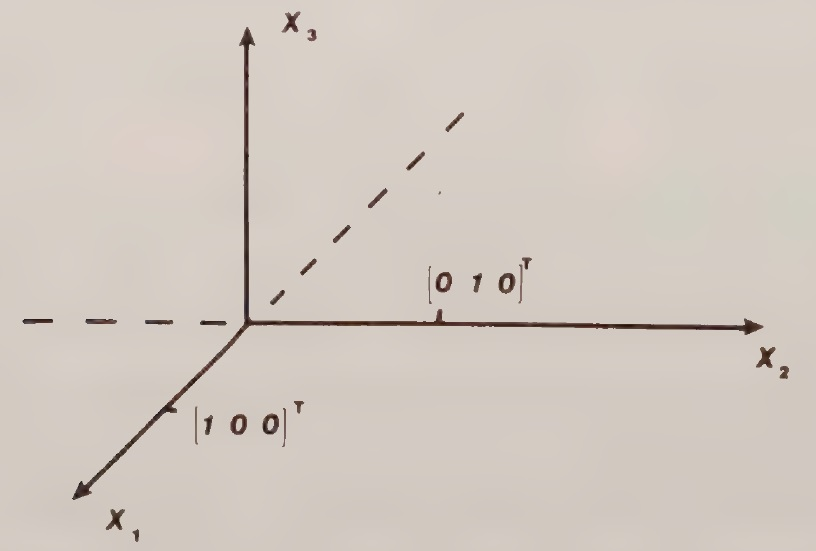
\includegraphics[width=0.58\linewidth,height=0.55\textheight,keepaspectratio]{figures/mp-2026/p068-hulls-example.jpg}
\end{frame}

% Source PDF page 069. Proposition 4's ray-only characterization was not
% sufficient for a convex cone and is corrected to nonnegative-combination
% closure; the remaining statements reproduce the source.
\begin{frame}{Affine \& Convex Sets}
  \footnotesize
  \begin{itemize}
    \item Proposition 1: For any nonempty set $S\subseteq\R^{n\times1}$,
      \begin{align*}
        S\subseteq X(S)\subseteq A(S)\subseteq L(S),\\
        S\subseteq X(S)\subseteq C(S)\subseteq L(S).
      \end{align*}
    \item Proposition 2: $S$ is a subspace of $\R^{n\times1}\Longleftrightarrow S=L(S)$
    \item Proposition 3: $S$ is an affine set $\Longleftrightarrow S=A(S)\Longleftrightarrow$ the line passing through any two distinct points in $S$ is a subset of $S$
    \item Proposition 4: $S$ is a convex cone $\Longleftrightarrow S=C(S)\Longleftrightarrow$ every nonnegative linear combination of points in $S$ belongs to $S$
    \item Proposition 5: $S$ is a convex set $\Longleftrightarrow S=X(S)\Longleftrightarrow$ the line segment connecting any two distinct points in $S$ is a subset of $S$
  \end{itemize}
\end{frame}

% Source PDF page 070
\begin{frame}{Affine \& Convex Sets}
  \small
  \begin{itemize}
    \item Proposition 6: A subset $S\subseteq\R^{n\times1}$ is affine $\Longleftrightarrow S-\vect{x}_0$ is a subspace of $\R^{n\times1}$, for every $\vect{x}_0\in S$
  \end{itemize}
  \begin{columns}[T,onlytextwidth]
    \begin{column}{0.52\textwidth}
      \begin{itemize}
        \item An affine set is just the translate of a subspace
        \item $\dim(S)=\dim(S-\vect{x}_0)$
        \item For any subset $T\subseteq\R^{n\times1}$, $\dim(T)=\dim(A(T))$
      \end{itemize}
    \end{column}
    \begin{column}{0.44\textwidth}
      \centering
      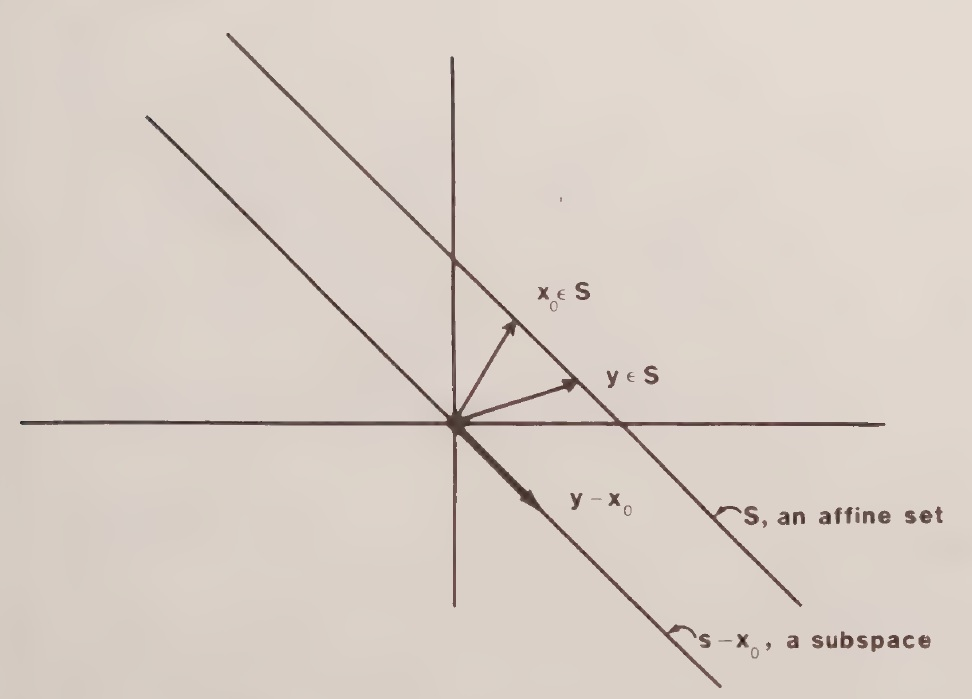
\includegraphics[width=\linewidth,height=0.48\textheight,keepaspectratio]{figures/mp-2026/p070-affine-translate.jpg}
    \end{column}
  \end{columns}
\end{frame}

\subsection{Hyperplanes, Polytopes, and Extreme Points}

% Source PDF page 071. The nonzero normal-vector condition is added because
% it is required in the definition of a hyperplane.
\begin{frame}{Affine \& Convex Sets}
  \small
  For $\vect{c}\ne\vect{0}$ and $\beta\in\R$:
  \begin{itemize}
    \item Hyperplane:
      \begin{equation*}H(\vect{c},\beta)=\{\vect{x}:\vect{c}^{\trans}\vect{x}=\beta\}\end{equation*}
    \item Upper half space:
      \begin{equation*}H^{+}(\vect{c},\beta)=\{\vect{x}:\vect{c}^{\trans}\vect{x}\ge\beta\}\end{equation*}
    \item Lower half space:
      \begin{equation*}H^{-}(\vect{c},\beta)=\{\vect{x}:\vect{c}^{\trans}\vect{x}\le\beta\}\end{equation*}
  \end{itemize}
  \centering
  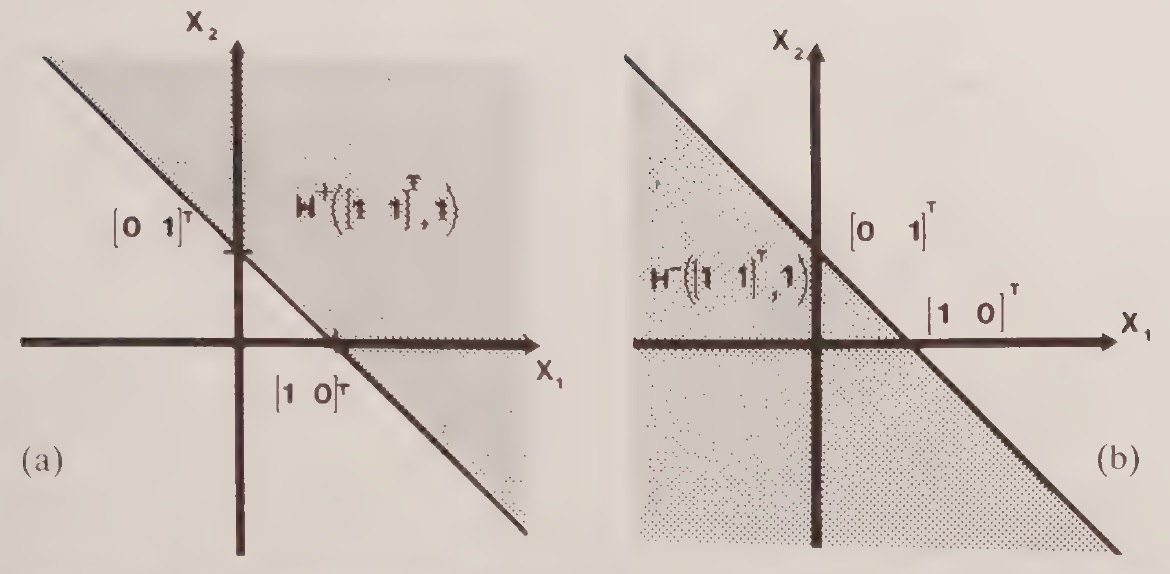
\includegraphics[width=0.38\linewidth,height=0.26\textheight,keepaspectratio]{figures/mp-2026/p071-hyperplane-halfspaces.jpg}
\end{frame}

% Source PDF page 072
\begin{frame}{Affine \& Convex Sets}
  \small
  \begin{columns}[T,onlytextwidth]
    \begin{column}{0.52\textwidth}
      \begin{itemize}
        \item Convex Polytope: $X(\{\vect{x}_1,\vect{x}_2,\ldots,\vect{x}_k\})$, $k<+\infty$
        \item Affinely Independent: $\{\vect{x}_0,\vect{x}_1,\ldots,\vect{x}_k\}$ is affinely independent $\Longleftrightarrow \{\vect{x}_1-\vect{x}_0,\vect{x}_2-\vect{x}_0,\ldots,\vect{x}_k-\vect{x}_0\}$ is linearly independent
        \item $k$-dimensional simplex: A convex polytope which is a convex hull of $k+1$ affinely independent vectors
      \end{itemize}
    \end{column}
    \begin{column}{0.44\textwidth}
      \centering
      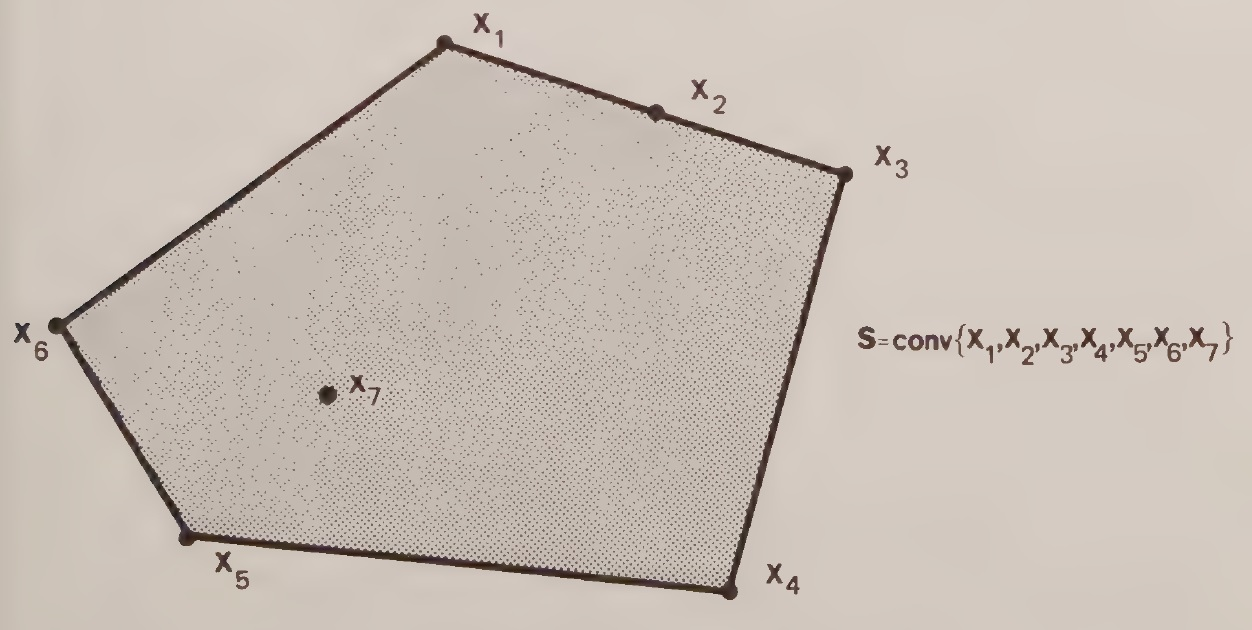
\includegraphics[width=\linewidth,height=0.52\textheight,keepaspectratio]{figures/mp-2026/p072-convex-polytope.jpg}
    \end{column}
  \end{columns}
\end{frame}

% Source PDF page 073
\begin{frame}{Affine \& Convex Sets}
  \centering
  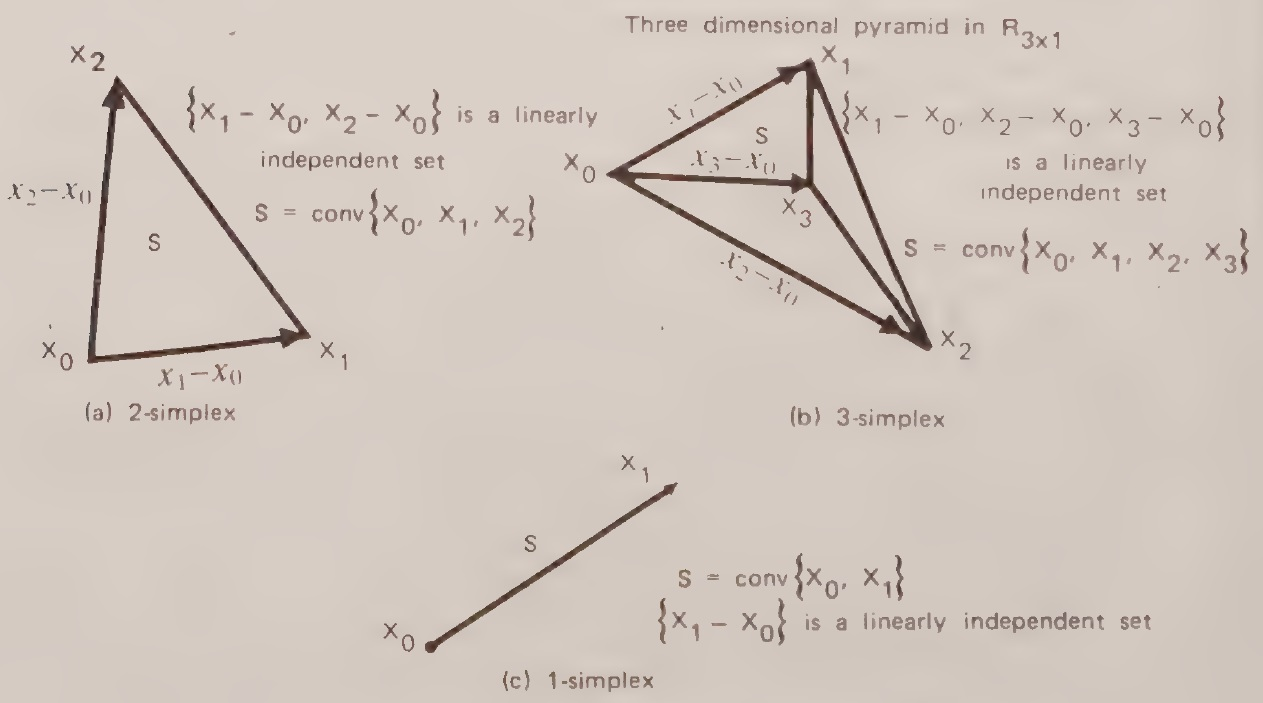
\includegraphics[width=0.76\linewidth,height=0.62\textheight,keepaspectratio]{figures/mp-2026/p073-simplex-examples.jpg}

  \smallskip
  Figure 1: (a) 2-simplex, (b) 3-simplex, (c) 1-simplex
\end{frame}

% Source PDF page 074. Source grammar ``pair of point'' corrected.
\begin{frame}{Affine \& Convex Sets}
  \small
  \begin{columns}[T,onlytextwidth]
    \begin{column}{0.57\textwidth}
      \begin{itemize}
        \item Extreme Point: $\vect{z}\in S$ (convex set) is an extreme point of $S$ $\Longleftrightarrow$ there does NOT exist distinct $\vect{x},\vect{y}\in S$ and $0<\alpha<1$ such that $\vect{z}=\alpha\vect{x}+(1-\alpha)\vect{y}$
        \item The vertices of any simplex are extreme points of the simplex
        \item The extreme points of a convex set $S$ are those NOT on the interior of any line segment connecting any other pair of points of $S$
      \end{itemize}
    \end{column}
    \begin{column}{0.39\textwidth}
      \centering
      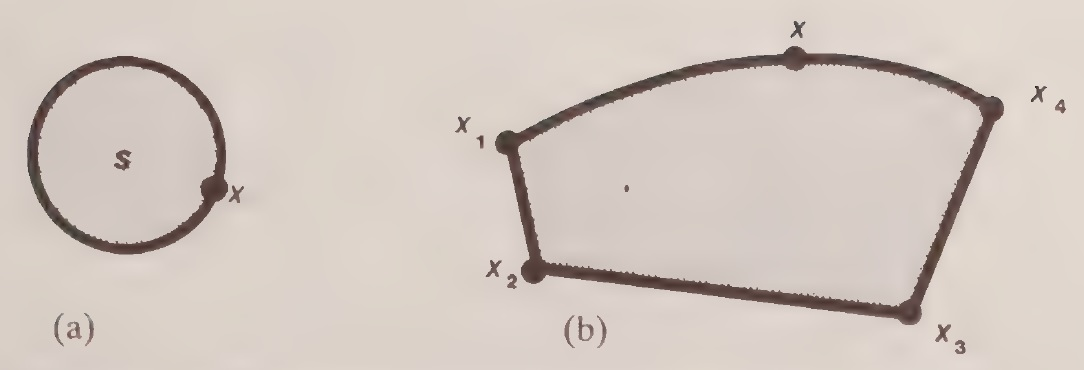
\includegraphics[width=\linewidth,height=0.43\textheight,keepaspectratio]{figures/mp-2026/p074-extreme-points.jpg}
    \end{column}
  \end{columns}
\end{frame}

\section{Linear Programming Problem}
\subsection{Feasible Polyhedra}

% Source PDF page 075
\begin{frame}{Linear Programming Problem}
  \begin{itemize}
    \item Original expression
      \begin{equation*}
        \min\ c_1x_1+\ldots+c_nx_n
      \end{equation*}
      subject to
      \begin{align*}
        a_{1,1}x_1+\ldots+a_{1,n}x_n&\le b_1,\\
        &\vdots\\
        a_{m,1}x_1+\ldots+a_{m,n}x_n&\le b_m,
      \end{align*}
      and
      \begin{equation*}
        \forall\ x_i\ge0.
      \end{equation*}
  \end{itemize}
\end{frame}

% Source PDF page 076
\begin{frame}{Linear Programming Problem}
  \begin{itemize}
    \item Equivalent expression:
      \begin{equation*}
        \min\ \vect{c}^{\trans}\vect{x}
      \end{equation*}
      subject to
      \begin{align*}
        A\vect{x}=A^{(1)}x_1+A^{(2)}x_2+\ldots+A^{(n)}x_n&\le\vect{b},\\
        \vect{x}&\ge\vect{0}.
      \end{align*}
    \item Set of feasible solutions: $F=\{\vect{x}:A\vect{x}\le\vect{b}\ \cap\ \vect{x}\ge\vect{0}\}$
  \end{itemize}
\end{frame}

% Source PDF page 077. ``half planes'' corrected to ``half spaces.''
\begin{frame}{Linear Programming Problem}
  \small
  \begin{itemize}
    \item Proposition 7: The set of feasible solution, $F$, to the linear programming problem is a convex set
    \item Proof: Let $\vect{x}_1,\vect{x}_2\in F$, $\alpha\in[0,1]$, check the convex combination $\vect{z}=\alpha\vect{x}_1+(1-\alpha)\vect{x}_2$. Does $\vect{z}\in F$?
    \item $F=\left(\bigcap_{i=1}^{m}\{\vect{x}:A_{(i)}\vect{x}\le b_i\}\right)
      \cap\left(\bigcap_{i=1}^{n}\{\vect{x}:x_i\ge0\}\right)$
    \item Convex polyhedron: Intersection of finite number of half spaces
    \item Convex polytope $\Longrightarrow$ Convex polyhedron; the converse does not hold in general
  \end{itemize}
\end{frame}

% Source PDF page 078
\begin{frame}{Linear Programming Problem}
  \begin{columns}[T,onlytextwidth]
    \begin{column}{0.49\textwidth}
      \centering
      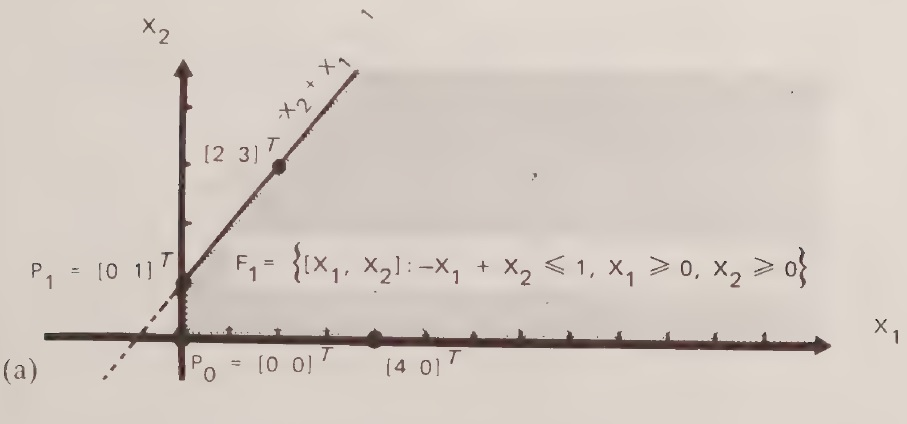
\includegraphics[width=\linewidth,height=0.53\textheight,keepaspectratio]{figures/mp-2026/p078-unbounded-polyhedron.jpg}\\
      \small (a) An unbounded convex polyhedron that is NOT a convex polytope
    \end{column}
    \begin{column}{0.49\textwidth}
      \centering
      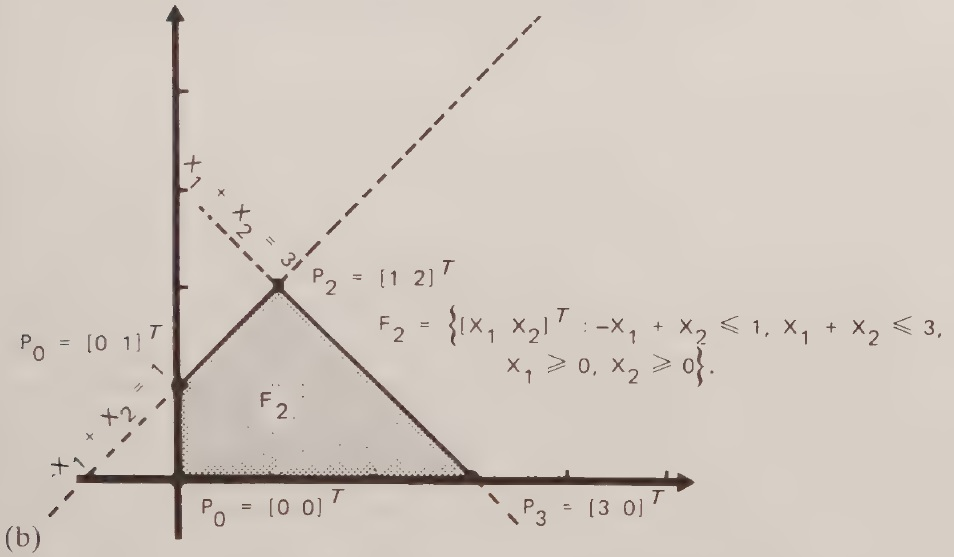
\includegraphics[width=\linewidth,height=0.53\textheight,keepaspectratio]{figures/mp-2026/p078-bounded-polytope.jpg}\\
      \small (b) A bounded convex polyhedron is a convex polytope
    \end{column}
  \end{columns}
\end{frame}

% Source PDF page 079. The source incorrectly required the finite point set
% to be the set of extreme points; the standard finite-generation statement
% below also covers polyhedra with lineality and no extreme points.
\begin{frame}{Linear Programming Problem}
  \small
  \begin{block}{Finite Basis Theorem}
    Let $F=\{\vect{x}\in\R^{n\times1}:A\vect{x}\le\vect{b}\}$ be a nonempty convex polyhedron. Then there exist finite sets $\{\vect{x}_1,\ldots,\vect{x}_d\}$ and $\{\vect{y}_1,\ldots,\vect{y}_{\ell}\}$ such that
    \begin{equation*}
      F=X(\{\vect{x}_1,\ldots,\vect{x}_d\})+C(\{\vect{y}_1,\ldots,\vect{y}_{\ell}\}),
    \end{equation*}
    i.e.,
    \begin{equation*}
      F=\left\{\sum_{i=1}^{d}\alpha_i\vect{x}_i+\sum_{j=1}^{\ell}\beta_j\vect{y}_j:
      \alpha_i\ge0,\ \beta_j\ge0,\ \sum_{i=1}^{d}\alpha_i=1\right\}.
    \end{equation*}
  \end{block}
\end{frame}

% Source PDF page 080
\begin{frame}{Linear Programming Problem}
  \centering
  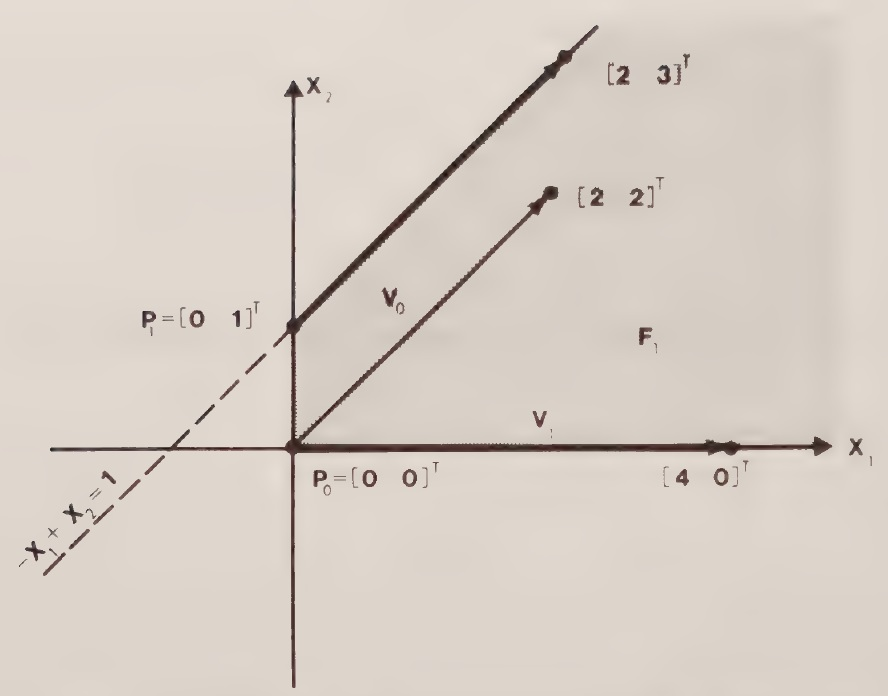
\includegraphics[width=0.56\linewidth,height=0.54\textheight,keepaspectratio]{figures/mp-2026/p080-finite-basis-decomposition.jpg}

  \footnotesize
  Figure 3: $F_2=X(\{\vect{p}_0,\vect{p}_1\})+C(\{\vect{v}_0,\vect{v}_1\})$, i.e., $F_2$ can be expressed as
  $\vect{x}=\alpha_0\vect{p}_0+\alpha_1\vect{p}_1+\beta_0\vect{v}_0+\beta_1\vect{v}_1$, where
  $\alpha_0\ge0$, $\alpha_1\ge0$, $\beta_0\ge0$, $\beta_1\ge0$ and $\alpha_0+\alpha_1=1$
\end{frame}

% ========== 第81页 ==========
\subsection{The Simplex Method}
\begin{frame}{Theorem on Bounded Linear Functions}
\textbf{Theorem} \\
If linear function \(f(\mathbf{x}) = \mathbf{c}^{T}\mathbf{x}\) is bounded from below/above (i.e., \(f(\mathbf{x})\geq \mu)\) over the convex polyhedron \(F = \{\mathbf{x}: \mathbf{A}\mathbf{x}\leq \mathbf{b}\}\) , then \(f(\mathbf{x})\) obtains a minimum/maximum over \(F\) , which occurs at one of the extreme points of \(F\) \\
Proof: If \(\mathbf{x}\in F\) , then \(\mathbf{x} = \sum_{i = 1}^{d}\alpha_{i}\mathbf{x}_{i} + \sum_{i = 1}^{\ell}\beta_{i}\mathbf{y}_{i}\) , where \(\alpha_{i}\geq 0\) \(\beta_{i}\geq 0\) \(\sum_{i = 1}^{d}\alpha_{i} = 1\) . Let \(f(\mathbf{x}_{k}) = \min \{f(\mathbf{x}_{1}),\ldots ,f(\mathbf{x}_{d})\}\) \\
\[
f(\mathbf{x}) = f\left(\sum_{i = 1}^{d}\alpha_{i}\mathbf{x}_{i} + \sum_{i = 1}^{\ell}\beta_{i}\mathbf{y}_{i}\right) = \sum_{i = 1}^{d}\alpha_{i}f(\mathbf{x}_{i}) + \sum_{i = 1}^{\ell}\beta_{i}f(\mathbf{y}_{i}) \geq \sum_{i = 1}^{d}\alpha_{i}f(\mathbf{x}_{i}) \geq \sum_{i = 1}^{d}\alpha_{i}f(\mathbf{x}_{k}) = f(\mathbf{x}_{k})\sum_{i = 1}^{d}\alpha_{i} = f(\mathbf{x}_{k})
\]
\end{frame}

% ========== 第82页 ==========
\begin{frame}{Quiz: Minimize Linear Function}
- Minimize \(f(x_1, x_2) = -x_1 + x_2\), subject to the constraints
\begin{align*}
-x_1 + 2x_2 & \le 10 \\
5x_1 + 3x_2 & \le 41 \\
2x_1 - 3x_2 & \le 8 \\
x_1 & \ge 0 \\
x_2 & \ge 0
\end{align*}
\end{frame}

% ========== 第83页 ==========
\begin{frame}{Quiz: Matrix Notation}
- Minimize \(f(x) = c^T x\), subject to \(Ax \leq b\), \(x \geq 0\) \\
Note that \(\mathbf{x} = [x_1, x_2]^T\), \(\mathbf{c} = [-1, 1]^T\), \(\mathbf{b} = [10, 41, 8]^T\) \\
\textit{[此处为线性规划可行域及等值线的几何插图]}
\end{frame}

% ========== 第84页 ==========
\begin{frame}{LP Problem: Slack Variables}
Finding the optimal solution to the LPP \(\longrightarrow\) Finding extreme points of the convex polyhedron of \(F\) \\
- Change inequality constraints to equality constraints via slack variables
\begin{align*}
a_{1,1}x_{1} + \ldots +a_{1,n}x_{n} + x_{n + 1} &= b_{1} \\
a_{2,1}x_{1} + \ldots +a_{2,n}x_{n} + x_{n + 2} &= b_{2} \\
\vdots & \vdots \\
a_{m,1}x_{1} + \ldots +a_{m,n}x_{n} + x_{n + m} &= b_{m}
\end{align*}
where \(x_{i} \geq 0, \forall i \in \{1, 2, \ldots , n + m\}\)
\end{frame}

% ========== 第85页 ==========
\begin{frame}{LP Problem: Standard Form}
1. \(\min \hat{c}^{T}\hat{x}\) , \(\hat{A}\hat{x} = \mathbf{b}\) , \(\hat{x}\geq 0\) , where \(\hat{c} = [c_{1},\ldots ,c_{n},0,\ldots ,0]^{T}\) \\
2. Feasible set: \(\hat{F} = \left\{\hat{x}\in \mathbf{R}_{(n + m)\times 1}:\hat{A}\hat{x} = \mathbf{b},\hat{x}\geq 0\right\}\) \\
3. Coefficient matrix 
\[
\hat{A} = \begin{bmatrix} a_{1,1} & \ldots & a_{1,n} & 1 & 0 & \ldots & 0\\ a_{2,1} & \ldots & a_{2,n} & 0 & 1 & \ldots & 0\\ \vdots & \ddots & \vdots & \vdots & \vdots & \ddots & \vdots \\ a_{m,1} & \ldots & a_{m,n} & 0 & 0 & \ldots & 1 \end{bmatrix} = \left[ \mathbf{A}|\mathbf{I}_{m} \right]
\]
\end{frame}

% ========== 第86页 ==========
\begin{frame}{Mapping between F and $\hat{F}$}
- Define a function \(\sigma : F \to \hat{F}\), i.e.,
\[
\sigma(\mathbf{x}) = \hat{\mathbf{x}} = \begin{bmatrix} \mathbf{x} \\ \mathbf{b} - \mathbf{A}\mathbf{x} \end{bmatrix}
\]
- Proposition 8: \(\sigma(\cdot)\) is a one-to-one mapping that preserves convex combinations of vectors, i.e.,
\[
\sigma(\alpha x + (1 - \alpha)y) = \alpha\sigma(x) + (1 - \alpha)\sigma(y)
\]
- Proposition 9: \(\mathbf{x}\) is an extreme point of \(F \iff \hat{\mathbf{x}}\) is an extreme point of \(\hat{F}\)
\end{frame}

% ========== 第87页 ==========
\begin{frame}{Example: Mapping $\sigma$}
\[
F = \{[x_1, x_2]^T : x_1 + x_2 \le 1, x_1 \ge 0, x_2 \ge 0\}
\]
\[
\hat{F} = \{[x_1, x_2, x_3]^T : x_1 + x_2 + x_3 = 1, x_1 \ge 0, x_2 \ge 0, x_3 \ge 0\}
\]
\[
\sigma([1, 0]^T) = [1, 0, 0]^T, \quad \sigma([0, 1]^T) = [0, 1, 0]^T, \quad \sigma([0, 0]^T) = [0, 0, 1]^T
\]
\end{frame}

% ========== 第88页 ==========
\begin{frame}{Theorem on Extreme Points of $\hat{F}$}
\textbf{Theorem} \\
If \(\hat{x}\) is an extreme point of \(\hat{F}\) and \(\Delta = \{j: |\hat{x}_j| > 0\}\) , then the columns \(\left\{\hat{A}^{(j)}: j \in \Delta\right\}\) is linearly independent \\
If
\begin{itemize}
    \item (a) \(\left\{\hat{A}^{(i)}: i \in \Delta\right\}\) is some collection of \(m\) linearly independent columns of \(\hat{A}\)
    \item (b) \(\mathbf{B}\) is the matrix whose columns are \(\left\{\hat{A}^{(i)}: i \in \Delta\right\}\)
    \item (c) \(\mathbf{x}^*\) is a solution to \(\mathbf{B}\mathbf{x} = \mathbf{b}, \mathbf{x} \geq \mathbf{0}\)
\end{itemize}
Then the vector \(\hat{x}\) whose \(i\) - th entry
\[
[\hat{x}]_i = \left\{ \begin{array}{ll} 0, & i \notin \Delta \\ {[\mathbf{x}^*]_i}, & i \in \Delta \end{array} \right.
\]
is an extreme point of \(\hat{F}\)
\end{frame}

% ========== 第89页 ==========
\begin{frame}{Example: Reformulation with Slack}
- Minimize \(f(x_1, x_2) = -x_1 + x_2\), subject to the constraints
\begin{align*}
-x_1 + 2x_2 & \leq & 10 \\
5x_1 + 3x_2 & \leq & 41 \\
2x_1 - 3x_2 & \leq & 8 \\
x_1 & \geq & 0 \\
x_2 & \geq & 0
\end{align*}
- Reformulation: \(\min \{-x_1 + x_2 + 0 \cdot x_3 + 0 \cdot x_4 + 0 \cdot x_5\}\), subject to \(x_i \geq 0, \forall i \in \{1, \ldots, 5\}\), and
\[
\begin{bmatrix}
-1 & 2 & 1 & 0 & 0 \\
5 & 3 & 0 & 1 & 0 \\
2 & -3 & 0 & 0 & 1
\end{bmatrix}
\begin{bmatrix}
x_1 \\
x_2 \\
x_3 \\
x_4 \\
x_5
\end{bmatrix}
=
\begin{bmatrix}
10 \\
41 \\
8
\end{bmatrix}
\]
\end{frame}

% ========== 第90页 ==========
\begin{frame}{Example: Finding Extreme Points}
At most \(\binom{5}{3} = 10\) sets of three linearly independent columns in the coefficient matrix \\
Select the first three columns \((x_{4} = x_{5} = 0)\)
\[
\mathbf{B} = [\hat{\mathbf{A}}^{(1)},\hat{\mathbf{A}}^{(2)},\hat{\mathbf{A}}^{(3)}]
\]
\(x_{1} = 7,x_{2} = 2,x_{3} = 13\) all nonnegative \(\mathbf{x}^{*} = [7,2,13]^{T}\) \(\rightarrow \hat{\mathbf{x}} = [7,2,13,0,0]^{T}\) is an extreme point of \(\hat{F}\) \(\rightarrow [7,2]^{T}\) is an extreme point of \(F\)
\end{frame}

% ========== 第91页 ==========
\begin{frame}{Example: Invalid Basis}
- Select \(\hat{A}^{(1)}, \hat{A}^{(2)}, \hat{A}^{(4)}\) (\(x_3=x_5=0\))
\[
\mathbf{B} = [\hat{\mathbf{A}}^{(1)},\hat{\mathbf{A}}^{(2)},\hat{\mathbf{A}}^{(4)}]
= \begin{bmatrix}
-1 & 2 & 0 \\
5 & 3 & 1 \\
2 & -3 & 0
\end{bmatrix}
\]
Solving \(\mathbf{B}\mathbf{x}=\mathbf{b}\) gives \(x_1=46\), \(x_2=28\), \(x_4=-273\) (negative), so \([46,28,0,-273,0]^T\notin\hat{F}\), hence \([46,28]^T\) is NOT an extreme point of \(F\).
\end{frame}

% ========== 第92页 ==========
\begin{frame}{Primal Simplex: Equality Form}
Any LLP can be expressed as:
\[
\min \mathbf{c}^T\mathbf{x}\mathrm{~subject~to~}\mathbf{A}\mathbf{x} = \mathbf{b}\mathrm{~and~}\mathbf{x}\geq \mathbf{0}
\]
\(\mathbf{A} \in \mathbf{R}_{m\times n}\) \(\mathbf{x}\in \mathbf{R}_{n\times 1}\) , and \(\operatorname {rank}(\mathbf{A}) = m\leq n\) \\
All the constraints are equality constraints \\
Each \(\mathbf{x}_i\) is restricted to be nonnegative \\
Equivalent problem with \(z_{o} = \mathbf{c}^{T}\mathbf{x}\) : Finding a solution \(\mathbf{x}\in \mathbf{R}_{n\times 1}\) and \(z_{o}\in \mathcal{R}\)
\[
\begin{array}{rcl}{\mathbf{A}\mathbf{x}} & = & {\mathbf{b}}\\ {-\mathbf{c}^{T}\mathbf{x} + z_{o}} & = & {0} \end{array}
\]
for \(\mathbf{x}\geq \mathbf{0}\) and \(z_{o}\) is minimal
\end{frame}

% ========== 第93页 ==========
\begin{frame}{Primal Simplex: Matrix Equation}
Matrix equation \\
Assume \(\operatorname{rank}(\mathbf{A}) = m\):
\[
\mathbf{A} = \underbrace{\left[\mathbf{A}^{(1)},\ldots,\mathbf{A}^{(m)},\mathbf{A}^{(m + 1)},\ldots,\mathbf{A}^{(n)}\right]}_{\coloneqq \mathbf{B}} = \mathbf{D}
\]
Initial matrix for the problem:
\textit{[此处为初始矩阵的示意图，包含 A, b, c, z_o 的分块结构]}
\end{frame}

% ========== 第94页 ==========
\begin{frame}{Primal Simplex: Initial Tableau}
- Left multiplying the initial matrix by:
\textit{[此处为矩阵乘法示意图]}
- It results simplex tableau:
\textit{[此处为单纯形表形式的矩阵示意图]}
- Can be alternatively done by a sequence of elementary row operations
\end{frame}

% ========== 第95页 ==========
\begin{frame}{Primal Simplex: Simplex Tableau}
Above augmented matrix represents the linear system:
\[
\begin{bmatrix}
\mathbf{I}_m & \mathbf{B}^{-1}\mathbf{D} & \mathbf{0} \\
\mathbf{0}^T & \mathbf{c}_B^T\mathbf{B}^{-1}\mathbf{D} - \mathbf{c}_D^T & 1
\end{bmatrix}
\begin{bmatrix}
\mathbf{x}_B \\
\mathbf{x}_D \\
z_o
\end{bmatrix}
=
\begin{bmatrix}
\mathbf{B}^{-1}\mathbf{b} \\
\mathbf{c}_B^T\mathbf{B}^{-1}\mathbf{b}
\end{bmatrix}
\]
\[\begin{cases}
\mathbf{x}_B + \mathbf{B}^{-1}\mathbf{D}\mathbf{x}_D = \mathbf{B}^{-1}\mathbf{b} \\
(\mathbf{c}_B\mathbf{B}^{-1}\mathbf{D} - \mathbf{c}_D^T)\mathbf{x}_D + z_o = \mathbf{c}_B^T\mathbf{B}^{-1}\mathbf{b}
\end{cases}\]
If \(\mathbf{B}^{-1}\mathbf{b} \ge 0\), \(\mathbf{c}_B\mathbf{B}^{-1}\mathbf{D} - \mathbf{c}_D^T \le 0^T\):
\[\begin{cases}
z_o = \mathbf{c}_B^T \mathbf{B}^{-1} \mathbf{b} \\
\mathbf{x}_B = \mathbf{B}^{-1} \mathbf{b} \\
\mathbf{x}_D = \mathbf{0}
\end{cases}\]
\end{frame}

% ========== 第96页 ==========
\begin{frame}{Example: Primal Simplex}
\textbf{Question:}
\[
\min -2x_1 - x_2 + 2x_3
\]
subject to
\[\begin{array}{rcl} x_1 + x_3 & = & 4 \\ -2x_1 + x_2 & = & 8 \\ x_1 & \geq & 0 \\ x_2 & \geq & 0 \\ x_3 & \geq & 0 \end{array}\]
\end{frame}

% ========== 第97页 ==========
\begin{frame}{Example: Basis Selection}
\textbf{Solution:} By elementary row operations,
\textit{[此处为包含增广矩阵的单纯形表]}
In above, \(\mathbf{B} = [\mathbf{A}^{(3)},\mathbf{A}^{(2)}]\)
\end{frame}

% ========== 第98页 ==========
\begin{frame}{Theorem 1: Optimality Condition}
\textbf{Theorem 1:} Solution for \(\min \mathbf{c}^T\mathbf{x}\) subject to \(\mathbf{A}\mathbf{x} = \mathbf{b}\) and \(\mathbf{x} \geq \mathbf{0}\) \\
If \(\mathbf{B}^{-1}\mathbf{b} \geq 0\) and \(\mathbf{c}_B\mathbf{B}^{-1}\mathbf{D} - \mathbf{c}_D^T \leq \mathbf{0}^T\), then the feasible solution
\[
\mathbf{x}_o = \begin{bmatrix} \mathbf{x}_B \\ \mathbf{x}_D \end{bmatrix} := \begin{bmatrix} \mathbf{B}^{-1}\mathbf{b} \\ \mathbf{0} \end{bmatrix}
\]
is optimal, and \(z_o = \min \mathbf{c}^T\mathbf{x} = \mathbf{c}^T\mathbf{x}_o = \mathbf{c}_B^T\mathbf{B}^{-1}\mathbf{b}\) \\
\textbf{Proof:} Suppose an \textbf{arbitrary} feasible solution \(\mathbf{A}\bar{\mathbf{x}} = \mathbf{b}\) and \(\bar{\mathbf{x}} \geq \mathbf{0}\)
\begin{align*}
\mathbf{b} &= \mathbf{A}\bar{\mathbf{x}} = [\mathbf{B},\mathbf{D}]\bar{\mathbf{x}} = \mathbf{B}[\mathbf{I}_m,\mathbf{B}^{-1}\mathbf{D}]\bar{\mathbf{x}} = \mathbf{B}\mathbf{x}_B \\
&\Rightarrow \mathbf{B}[\mathbf{x}_B - [\mathbf{I}_m,\mathbf{B}^{-1}\mathbf{D}]\bar{\mathbf{x}}] = \mathbf{0} \\
&\Rightarrow \mathbf{x}_B = [\mathbf{I}_m,\mathbf{B}^{-1}\mathbf{D}]\bar{\mathbf{x}} \\
&\Rightarrow \mathbf{c}_B^T\mathbf{x}_B = [\mathbf{c}_B^T,\mathbf{c}_B^T\mathbf{B}^{-1}\mathbf{D}]\bar{\mathbf{x}} \\
&\leq [\mathbf{c}_B^T,\mathbf{c}_D^T]\bar{\mathbf{x}} = \mathbf{c}^T\bar{\mathbf{x}}
\end{align*}
\(\mathbf{c}_B^T\mathbf{x}_B\) is the minimal value for the problem, and \(\mathbf{x}_o\) is optimal.
\end{frame}

% ========== 第99页 ==========
\begin{frame}{Basic Solutions and BFS}
- Basic solution of \(\mathbf{A}\mathbf{x} = \mathbf{b}\):
\[
\mathbf{x}_B = \mathbf{B}^{-1}\mathbf{b}, \quad \mathbf{x}_D = \mathbf{0}
\]
- Basis matrix: the nonsingular matrix \(\mathbf{B}\) \\
- Admissible basis: \(\mathbf{A}^{(1)},\ldots ,\mathbf{A}^{(m)}\) \\
- Basic feasible solution (BFS): a basic solution that is feasible \\
- Nondegenerate BFS: A BFS for which \(\mathbf{x}_B = \mathbf{B}^{-1}\mathbf{b} > 0\) \\
- Theorem 1 gives a sufficient condition, i.e., \(\mathbf{c}_B\mathbf{B}^{-1}\mathbf{D} - \mathbf{c}_D^T \leq \mathbf{0}^T\), for a BFS \(\mathbf{x}_B = \mathbf{B}^{-1}\mathbf{b} > 0\), and \(\mathbf{x}_D = \mathbf{0}^T\) to be an optimal solution.
\end{frame}

% ========== 第100页 ==========
\begin{frame}{Feasible, Basic, and BFS}
- Feasible Solution: "Qualified", wide range candidates
\[
\hat{A}\hat{x} = \mathbf{b}, \quad \hat{x}\geq 0
\]
- Basic Solution: "Simple \& Efficient", not necessarily feasible
\[
\hat{A}\hat{x} = \mathbf{b}, \quad \mathbf{x}_D = \mathbf{0}
\]
- BFS: "Key candidates" for optimal
\[
\hat{A}\hat{x} = \mathbf{b}, \quad \mathbf{x}_D = \mathbf{0}, \quad \hat{x}\geq 0
\]
\end{frame}

% ========== 第101页 ==========
\begin{frame}{Example: LP with Slack}
\textbf{Question:} \(\min 10x_1 + 18x_2\) subject to
\begin{align*}
5x_1 + 2x_2 &\leq 170 \\
2x_1 + 3x_2 &\leq 100 \\
x_1 + 5x_2 &\leq 150 \\
x_i &\geq 0, \forall i \in \{1, 2\}
\end{align*}
\textbf{Reformation:}
\begin{align*}
5x_1 + 2x_2 + x_3 &= 170 \\
2x_1 + 3x_2 + x_4 &= 100 \\
x_1 + 5x_2 + x_5 &= 150 \\
x_i &\geq 0, \forall i \in \{1, 2, ..., 5\}
\end{align*}
\end{frame}

% ========== 第102页 ==========
\begin{frame}{Example: Geometric Interpretation}
\textit{[此处为不等式约束围成的多边形的几何插图]}
基本解(10个): \(O, A, B, E, F, G, H, I\) \\
基本可行解(5个): \(O, A, B, C, E\) \\
最优解(1个): \(C\)
\end{frame}

% ========== 第103页 ==========
\begin{frame}{Simplex Tableau Details}
\textbf{The Primal Simplex Procedure} \\
Simplex Tableau:
\[
\begin{bmatrix}
\mathbf{I}_m & \mathbf{B}^{-1}\mathbf{D} & \mathbf{0} & \mathbf{B}^{-1}\mathbf{b} \\
\mathbf{0}^T & \mathbf{c}_B^T\mathbf{B}^{-1}\mathbf{D} - \mathbf{c}_D^T & 1 & \mathbf{c}_B^T\mathbf{B}^{-1}\mathbf{b}
\end{bmatrix}
\]
\(X_B \triangleq [\mathbf{I}_m, \mathbf{B}^{-1}\mathbf{D}]\)
\[
X_B = \begin{bmatrix} 1 & 0 & \cdots & 0 & x_{1,m+1} & \cdots & x_{1,j} & \cdots & x_{1,n} \\ 0 & 1 & \cdots & 0 & x_{2,m+1} & \cdots & x_{2,j} & \cdots & x_{2,n} \\ \vdots & \vdots & \ddots & \vdots & \vdots & \vdots & \vdots & \ddots & \vdots \\ 0 & 0 & \cdots & 1 & x_{m,m+1} & \cdots & x_{m,j} & \cdots & x_{m,n} \end{bmatrix}
\]
\(z_j \triangleq c_B^T \mathbf{B}^{-1} \mathbf{A}^{(j)}, c_j \triangleq [\mathbf{c}]_j, \forall j = 1, \ldots, n\)
\[
z_j - c_j = \begin{cases} 0 & j = 1, \ldots, m \\ {[c_B^T \mathbf{B}^{-1} \mathbf{D} - c_D^T]_j} & j = m+1, \ldots, n \end{cases}
\]
\end{frame}

% ========== 第104页 ==========
\begin{frame}{Theorem 2: Unboundedness}
\textbf{Theorem 1:} If \(z_j - c_j \leq 0\), \(\forall j = 1, \ldots , n\), the BFS \(\{x_B = \mathbf{B}^{-1} \mathbf{b} \geq 0, \mathbf{x}_D = 0\}\) is an optimal solution \\
What if \(z_j - c_j > 0\), for some \(j\) ? \\
\(\downarrow\) \\
\textbf{Theorem 2:} If there exists a \(j\) so that \(z_j - c_j > 0\) and each \(x_{i,j} \leq 0\), then the LLP
\[
\min \mathbf{c}^T \mathbf{x} \text{ subject to } \mathbf{A} \mathbf{x} = \mathbf{b} \text{ and } \mathbf{x} \geq \mathbf{0}
\]
has an unbounded minimum over \(F\)
\end{frame}

% ========== 第105页 ==========
\begin{frame}{Theorem 3 \& 4: Pivoting and Optimality}
\textbf{Theorem 3} \\
If there exists a \(j\) so that \(z_{j} - c_{j} > 0\) , and if some \(x_{i,j} > 0\) , then by pivoting at the element \(x_{k,j}\) , a new basic feasible solution is generated that does not increase the value of \(z_{o}\) . Note that \(k\) is selected such that
\[
\theta \triangleq \frac{[\mathbf{B}^{-1}\mathbf{b}]_{k}}{x_{k,j}} = \min \left\{\frac{[\mathbf{B}^{-1}\mathbf{b}]_{i}}{x_{i,j}}:x_{i,j} > 0\right\}
\]
If \(\mathbf{B}^{- 1}\mathbf{b} > 0\) , i.e., the BFS \(\mathbf{x}_{B} = \mathbf{B}^{- 1}\mathbf{b}\) and \(\mathbf{x}_{D} = \mathbf{0}\) is nondegenerate, then the value of \(z_{o}\) decreases. \\
\textbf{Theorem 4} \\
If \(\mathbf{c}^{T}\mathbf{x}\) obtains a finite minimum over \(F\) , then the minimum occurs at a BFS of \(F\) (the minimum may occur at other places as well)
\end{frame}

% ========== 第106页 ==========
\begin{frame}{Example: Introducing Slack}
\textbf{Question} \\
\[
\min \mathbf{c}^T\mathbf{x}
\]
subject to
\begin{align*}
3x_1 + x_3 - x_4 &= 1 \\
7x_1 + x_2 - x_4 &= 0 \\
-8x_1 + x_4 &\leq 1 \\
x_i &\geq 0, \forall i
\end{align*}
\end{frame}

% ========== 第107页 ==========
\begin{frame}{Example: Augmented Form}
- Add a slack variable
\[
\min \mathbf{c}^T\mathbf{x}
\]
subject to
\textit{[此处为增广矩阵与常数的表达]}
\[
\mathbf{c} = [1, - 1, 2, - 3, 0]^T
\]
\end{frame}

% ========== 第108页 ==========
\begin{frame}{Example: Basis and BFS}
\textbf{Example 14}
\[
\begin{bmatrix}
3 & 0 & 1 & -1 & 0 & 0 & 1 \\
7 & 1 & 0 & -1 & 0 & 0 & 0 \\
-8 & 0 & 0 & -1 & 1 & 0 & 1 \\
-1 & 1 & -2 & -3 & -1 & 0 & 1
\end{bmatrix}
\]
Row operation: \(\mathbf{A}_{(4)} - (\mathbf{A}_{(2)} - 2\mathbf{A}_{(1)})\)
\[
\begin{bmatrix}
3 & 0 & 1 & -1 & 0 & 0 & 1 \\
7 & 1 & 0 & -1 & 0 & 0 & 0 \\
-8 & 0 & 0 & -1 & 1 & 0 & 1 \\
-2 & 0 & 0 & -2 & -1 & 1 & 2
\end{bmatrix}
\]
\(\mathbf{B} = [\mathbf{A}^{(3)}, \mathbf{A}^{(2)}, \mathbf{A}^{(5)}]\) is nonsingular \\
\(\mathbf{D} = [\mathbf{A}^{(1)}, \mathbf{A}^{(4)}]\) \\
BFS: \([x_3, x_2, x_5]^T = [1, 0, 1]^T, [x_1, x_4]^T = [0, 0]^T\) (degenerate)
\end{frame}

% ========== 第109页 ==========
\begin{frame}{Example: Pivot and Unboundedness}
\textbf{Example 14}
\[
\begin{bmatrix}
3 & 0 & 1 & -1 & 0 & 0 & 1 \\
7 & 1 & 0 & -1 & 0 & 0 & 0 \\
-8 & 0 & 0 & -1 & 0 & 1 & 1 \\
-2 & 0 & 0 & -2 & 0 & 1 & 2
\end{bmatrix}
\]
Row operations: \(\mathbf{A}_{(1)}+\mathbf{A}_{(3)}, \mathbf{A}_{(2)}+\mathbf{A}_{(3)}, \mathbf{A}_{(4)}-2\mathbf{A}_{(3)}\)
\[
\begin{bmatrix}
-5 & 0 & 1 & 0 & 1 & 0 & 2 \\
-1 & 1 & 0 & 0 & 1 & 0 & 1 \\
-8 & 0 & 0 & -1 & 0 & 1 & 1 \\
-14 & 0 & 0 & -2 & 0 & 1 & 0
\end{bmatrix}
\]
(1) Pivot in the 4th column, since \(z_4 - c_4 = 2 > 0\) \\
(2) \(\min \left\{ \frac{|\mathbf{B}^{-1}\mathbf{b}_i|}{x_{i,4}} : x_{i,4} > 0 \right\} = 1 \Rightarrow k = 3 \Rightarrow \text{pivoting } x_{3,4}\) \\
(3) \(\mathbf{B} = [\mathbf{A}^{(3)}, \mathbf{A}^{(2)}, \mathbf{A}^{(4)}]\) and \(\mathbf{D} = [\mathbf{A}^{(1)}, \mathbf{A}^{(5)}]\) \\
(4) BFS: \(x_3 = 2\), \(x_2 = 1\), \(x_4 = 1\), and \(x_1 = x_5 = 0\) \\
(5) \(z_1 - c_1 = 14\), \(x_{1,1} = -5\), \(x_{2,1} = -1\), and \(x_{3,1} = -8\), the LLP has an unbounded minimum (Theorem 2)
\end{frame}

% ========== 第110页 ==========
\begin{frame}{Example: Maximization to Minimization}
\textbf{Question}
\[
\max 2x_1 + x_2 + 3x_3
\]
subject to
\begin{align*}
x_1 + 3x_2 + 2x_3 & \leq 6 \\
-x_1 + x_2 - 3x_3 & \geq -9 \\
x_i & \geq 0, \quad \forall i
\end{align*}
\textbf{Transformation}
\[
\min -2x_1 - x_2 - 3x_3
\]
subject to
\begin{align*}
x_1 + 3x_2 + 2x_3 + x_4 & = 6 \\
x_1 - x_2 + 3x_3 + x_5 & = 9 \\
x_i & \geq 0, \quad \forall i
\end{align*}
\end{frame}

% ========== 第111页 ==========
\begin{frame}{Example: Simplex Iterations}
\textbf{Example 15}
\[
\begin{bmatrix}
1 & 3 & 2 & 1 & 0 & 0 & 6 \\
-1 & 1 & -3 & 0 & 1 & 0 & 9
\end{bmatrix}
\]
Row operations: \(\mathbf{A}_{(2)} - \frac{3}{2}\mathbf{A}_{(1)}\), \(\mathbf{A}_{(3)} - \frac{3}{2}\mathbf{A}_{(1)}\), \(\frac{1}{2}\mathbf{A}_{(1)}\)
\[
\begin{bmatrix}
\frac{1}{2} & \frac{3}{2} & 1 & \frac{1}{2} & 0 & 0 & 3 \\
-\frac{1}{2} & -\frac{7}{2} & 0 & -\frac{3}{2} & 1 & 0 & 0
\end{bmatrix}
\]
BSF: \(\mathbf{x} = [0,0,0,6,9]^T\), with admissible basis of \(\{\mathbf{A}^{(4)},\mathbf{A}^{(5)}\}\) \\
Pivot in the 3rd column, since \(z_3 - c_3 = 3 > 0\) \\
\(\theta = \min \left\{ \frac{|\mathbf{B}^{-1}\mathbf{b}|_i}{x_{i,3}} : x_{i,3} > 0 \right\} = \min \left\{ \frac{6}{2}, \frac{9}{3} \right\} = 3\), either pivoting \(x_{1,3}\) or \(x_{2,3}\)
\end{frame}

% ========== 第112页 ==========
\begin{frame}{Example: Degeneracy and Pivot}
\textbf{Example 15}
\[
\begin{bmatrix}
\frac{1}{2} & \frac{3}{2} & 1 & \frac{1}{2} & 0 & 0 & 3 \\
-\frac{1}{2} & -\frac{7}{2} & 0 & -\frac{3}{2} & 1 & 0 & 0
\end{bmatrix}
\]
Row operations: \(\mathbf{A}_{(2)} + \mathbf{A}_{(1)}\), \(\mathbf{A}_{(3)} - \mathbf{A}_{(1)}\), \(2\mathbf{A}_{(1)}\)
\[
\begin{bmatrix}
1 & 3 & 2 & 1 & 0 & 0 & 6 \\
0 & -4 & 1 & -1 & 1 & 0 & 3
\end{bmatrix}
\]
New BSF: \(\{\mathbf{A}^{(3)},\mathbf{A}^{(5)}\}, \mathbf{x} = [0,0,3,0,0]^T\) (degenerate) \\
Pivot in the 1st column, since \(z_1 - c_1 = \frac{1}{2} > 0\) \\
\(\theta = \min \left\{ \frac{|\mathbf{B}^{-1}\mathbf{b}|_i}{x_{i,1}} : x_{i,1} > 0 \right\} = \min \{6\} = 6\), pivoting \(x_{1,1}\)
\end{frame}

% ========== 第113页 ==========
\begin{frame}{Example: Optimal Solution}
\textbf{Example 15}
\[
\begin{bmatrix}
1 & 3 & 2 & 1 & 0 & 0 & 6 \\
0 & -4 & 1 & -1 & 1 & 0 & 3
\end{bmatrix}
\]
Row operation: \(\mathbf{A}_{(2)} - \mathbf{A}_{(1)}\)
\[
\begin{bmatrix}
1 & 3 & 2 & 1 & 0 & 0 & 6 \\
0 & -4 & -5 & -1 & -1 & 0 & -12
\end{bmatrix}
\]
New BSF: \(\{\mathbf{A}^{(1)},\mathbf{A}^{(5)}\}, \mathbf{x} = [6,0,0,0,3]^T\) \\
Since \(z_j - c_j \leq 0, \forall j\), then \(\mathbf{x} = [6,0,0,0,3]^T\) is the optimum, and \(z_o = -12\) (Theorem 1) \\
Original LLP: \(\max \{c^T x : x \in F\} = 12\), and \(x = [6, 0, 0]^T\)
\end{frame}

% ========== 第114页 ==========
\begin{frame}{Example: New Problem}
\textbf{Question} \\
\[
\min \mathbf{c}^T\mathbf{x}
\]
subject to
\begin{align*}
16x_{1} + 2x_{2} + x_{5} + 10x_{6} &= 4 \\
-x_{1} + x_{4} + x_{6} &= 0 \\
5x_{1} + 4x_{2} + x_{3} &= 8 \\
x_{i} &\geq 0, \quad \forall i
\end{align*}
where \(\mathbf{c} = [1, -1, 2, -3, 0, 0]^T\)
\end{frame}

% ========== 第115页 ==========
\begin{frame}{Example: Simplex Steps}
\textbf{Example 16}
\[
\begin{bmatrix}
16 & 2 & 0 & 0 & 1 & 10 & 0 & 4 \\
-1 & 0 & 0 & 1 & 0 & 1 & 0 & 0 \\
5 & 4 & 1 & 0 & 0 & 0 & 0 & 8 \\
-1 & -1 & -2 & -3 & 0 & 0 & 1 & 0
\end{bmatrix}
\]
\(\downarrow A_{(4)} + (A_{(1)} + A_{(2)} + A_{(3)})\)
\[
\begin{bmatrix}
16 & 2 & 0 & 0 & 1 & 10 & 0 & 4 \\
-1 & 0 & 0 & 1 & 0 & 1 & 0 & 0 \\
5 & 4 & 1 & 0 & 0 & 0 & 0 & 8 \\
19 & 5 & 0 & 0 & 0 & 10 & 1 & 12
\end{bmatrix}
\]
BSF: \(\mathbf{x} = [0, 0, 8, 0, 4, 0]^T\) (degenerate), with admissible basis of \(\{\mathbf{A}^{(5)}, \mathbf{A}^{(4)}, \mathbf{A}^{(3)}\}\) \\
Pivot in the 6th column, since \(z_6 - c_6 = 10 > 0\) \\
\(\theta = \min \{0, \frac{4}{10}\} = 0\), pivoting \(x_{2,6}\)
\end{frame}

% ========== 第116页 ==========
\begin{frame}{Example: Pivot Selection}
\textbf{Example 16}
\[
\begin{bmatrix}
16 & 2 & 0 & 0 & 1 & 10 & 0 & 4 \\
-1 & 0 & 0 & 1 & 0 & 1 & 0 & 0 \\
5 & 4 & 1 & 0 & 0 & 0 & 0 & 8 \\
19 & 5 & 0 & 0 & 0 & 10 & 1 & 12
\end{bmatrix}
\]
\(\downarrow A_{(1)} - 10A_{(2)}, \quad A_{(4)} - 10A_{(2)}\)
\[
\begin{bmatrix}
26 & 2 & 0 & -10 & 1 & 0 & 0 & 4 \\
-1 & 0 & 0 & 1 & 0 & 1 & 0 & 0 \\
5 & 4 & 1 & 0 & 0 & 0 & 0 & 8 \\
29 & 5 & 0 & -10 & 0 & 0 & 1 & 12
\end{bmatrix}
\]
BSF: \(\mathbf{x} = [0, 0, 8, 0, 0, 4]^T\) (degenerate), with admissible basis of \(\{\mathbf{A}^{(5)}, \mathbf{A}^{(6)}, \mathbf{A}^{(3)}\}\) \\
Pivot in the 2nd column, since \(z_2 - c_2 = 5 > 0\) \\
\(\theta = \min\{\frac{4}{2}, \frac{8}{4}\} = 2\), pivoting either \(x_{1,2}\) or \(x_{3,2}\)
\end{frame}

% ========== 第117页 ==========
\begin{frame}{Example: Further Pivoting}
\textbf{Example 16}
\[
\begin{bmatrix}
26 & 2 & 0 & -10 & 1 & 0 & 0 & 4 \\
-1 & 0 & 0 & 1 & 0 & 1 & 0 & 0 \\
5 & 4 & 1 & 0 & 0 & 0 & 0 & 8 \\
29 & 5 & 0 & -10 & 0 & 0 & 1 & 12
\end{bmatrix}
\]
\(\downarrow A_{(3)} - 2A_{(1)}, \quad A_{(4)} - \frac{5}{2}A_{(1)}, \quad \frac{1}{2}A_{(1)}\)
\[
\begin{bmatrix}
13 & 1 & 0 & -5 & \frac{1}{2} & 0 & 0 & 2 \\
-1 & 0 & 0 & 1 & 0 & 1 & 0 & 0 \\
-21 & 0 & 1 & 20 & -2 & 0 & 0 & 4 \\
-36 & 0 & 0 & 15 & -\frac{5}{2} & 0 & 1 & 2
\end{bmatrix}
\]
BSF: \(x = [0, 2, 0, 0, 0, 0]^T\) (degenerate), with admissible basis of \(\{\mathbf{A}^{(2)}, \mathbf{A}^{(6)}, \mathbf{A}^{(3)}\}\) \\
Pivot in the 4th column, since \(z_4 - c_4 = 15 > 0\) \\
\(\theta = \min\{\frac{0}{1}, \frac{0}{20}\} = 0\), pivoting either \(x_{2,4}\) or \(x_{3,4}\)
\end{frame}

% ========== 第118页 ==========
\begin{frame}{Example: Optimality Reached}
\textbf{Example 16}
\[
\begin{bmatrix}
13 & 1 & 0 & -5 & \frac{1}{2} & 0 & 0 & 2 \\
-1 & 0 & 0 & 1 & 0 & 1 & 0 & 0 \\
-21 & 0 & 1 & 20 & -2 & 0 & 0 & 4 \\
-36 & 0 & 0 & 15 & -\frac{5}{2} & 0 & 1 & 2
\end{bmatrix}
\]
\(\downarrow A_{(1)} + 5A_{(2)}, \quad A_{(3)} - 20A_{(2)}, \quad A_{(4)} - 15A_{(2)}\)
\[
\begin{bmatrix}
8 & 1 & 0 & 0 & \frac{1}{2} & 5 & 0 & 2 \\
-1 & 0 & 0 & 1 & 0 & 1 & 0 & 0 \\
-1 & 0 & 1 & 0 & -2 & -20 & 0 & 4 \\
-21 & 0 & 0 & 0 & -\frac{5}{2} & -15 & 1 & 2
\end{bmatrix}
\]
Since \(z_j - c_j \le 0, \forall j\), then \(\mathbf{x} = [0, 2, 0, 0, 0, 0]^T\) is the optimum, and \(z_o = 2\) (Theorem 1) \\
The admissible basis: \(\{\mathbf{A}^{(2)}, \mathbf{A}^{(4)}, \mathbf{A}^{(3)}\}\)
\end{frame}

% ========== 第119页 ==========
\begin{frame}{Example: Multiple Optima}
\textbf{Question:} Find several points \(\mathbf{x} = [x_1, x_2, x_3, x_4]^T\) that solve the problem
\[
\min 3x_1 + 2x_2 + 6x_3 + x_4
\]
subject to
\begin{align*}
x_1 + x_4 &= 4 \\
x_1 + x_2 + x_3 &= 5 \\
x_i &\geq 0, \forall i
\end{align*}
\end{frame}

% ========== 第120页 ==========
\begin{frame}{Example: Finding BFS}
\textbf{Example 17}
\[
\begin{bmatrix}
1 & 0 & 0 & 1 & 0 & 4 \\
1 & 1 & 1 & 0 & 0 & 5 \\
-3 & -2 & -6 & -1 & 1 & 0
\end{bmatrix}
\Rightarrow
\begin{bmatrix}
1 & 0 & 0 & 1 & 0 & 4 \\
1 & 1 & 1 & 0 & 0 & 5 \\
0 & 0 & -2 & -2 & 0 & 1
\end{bmatrix}
\]
BSF: \(\{\mathbf{A}^{(4)}, \mathbf{A}^{(2)}\}, \mathbf{x} = [0, 5, 0, 4]^T\) \\
Since \(z_j - c_j \leq 0, \forall j\), then \(\mathbf{x}_1 = [0, 5, 0, 4]^T\) is the optimum, and \(z_o = 14\) (Theorem 1)
\end{frame}

% ========== 第121页 ==========
\begin{frame}{Example: Alternative Optimal Solution}
\textbf{Example 17}
\[
\begin{bmatrix}
1 & 0 & 0 & 1 & 0 & 4 \\
1 & 1 & 1 & 0 & 0 & 5 \\
0 & 0 & -2 & -2 & 0 & 1
\end{bmatrix}
\Rightarrow
\mathbf{A}_{(2)} - \mathbf{A}_{(1)}
\begin{bmatrix}
1 & 0 & 0 & 1 & 0 & 4 \\
0 & 1 & 1 & -1 & 0 & 1 \\
0 & 0 & -2 & -2 & 0 & 1
\end{bmatrix}
\]
Consider \(z_1 - c_1 = 0\), \(\theta = \min\{\frac{4}{1}, \frac{5}{1}\} = 4\), pivoting \(x_{1,1}\) \\
BSF: \(\{\mathbf{A}^{(1)}, \mathbf{A}^{(2)}\}, \mathbf{x} = [4, 1, 0, 0]^T\) \\
Since \(z_j - c_j \le 0, \forall j\), then \(\mathbf{x}_2 = [4, 1, 0, 0]^T\) is also the optimum, and \(z_o = 14\) (Theorem 1)
\end{frame}

% ========== 第122页 ==========
\begin{frame}{Useful Points in Simplex}
Useful points when using the primal simplex procedure:
\begin{enumerate}
    \item \(z_0\) should never increase from one tableau to the next
    \item \(\mathbf{B}^{-1}\mathbf{b}\) should never contain negative components
    \item For each \(\mathbf{A}^{(j)}\) in the admissible basis, \(z_j - c_j = 0\)
\end{enumerate}
\end{frame}

% ========== 第123页 ==========
\begin{frame}{Artificial Variables Introduction}
To solve LLP with the primal simplex procedure, an initial BFS of \(F\) is required before setting up the first tableau. \\
This is possible after adding slack variables, \(\mathbf{A} = [a_{i,j}]\) contains \(\mathbf{I}_{m}\) \\
\textbf{Question:} What if \(\mathbf{A} = [a_{i,j}]\) does NOT contain \(\mathbf{I}_{m}\) ?
\end{frame}

% ========== 第124页 ==========
\begin{frame}{Artificial Variables Formulation}
\textbf{Question:}
\[
\min \quad c_1x_1 + \dots + c_nx_n + Mx_{n+1} + \dots + Mx_{n+m}
\]
subject to
\begin{align*}
a_{1,1}x_1 + \dots + a_{1,n}x_n + x_{n+1} &= b_1 \\
a_{2,1}x_1 + \dots + a_{2,n}x_n + x_{n+2} &= b_2 \\
\vdots & \vdots \\
a_{m,1}x_1 + \dots + a_{m,n}x_n + x_{n+m} &= b_m
\end{align*}
\[
x_1 \ge 0, \dots, x_n \ge 0, x_{n+1} \ge 0, \dots, x_{n+m} \ge 0
\]
\(M\): an unspecified large positive number \\
\(x_{n+1}, \dots, x_{n+m}\): artificial variables
\end{frame}

% ========== 第125页 ==========
\begin{frame}{Objective with Artificial Variables}
- The objective function:
\begin{align*}
f(\mathbf{y}) &= c_1y_1 + \dots +c_ny_n \\
\bar{f}(\bar{\mathbf{y}}) &= c_1y_1 + \dots +c_ny_n + My_{n+1} + \dots +My_{n+m}
\end{align*}
- The set of feasible solutions:
\begin{align*}
F &= \{\mathbf{y}\in \mathbf{R}_{n\times 1}:\mathbf{A}\mathbf{y} = \mathbf{b},\mathbf{y}\geq 0\} \\
\bar{F} &= \{\bar{\mathbf{y}}\in \mathbf{R}_{(n + m)\times 1}:[\mathbf{A},\mathbf{I}_m]\bar{\mathbf{y}} = \mathbf{b},\bar{\mathbf{y}}\geq 0\}
\end{align*}
- Specific solution:
\textit{[此处为人工变量构造的初始单纯形表格]}
\end{frame}

% ========== 第126页 ==========
\begin{frame}{Mapping between F and F̄}
\(p:F\rightarrow \bar{F}\) , i.e., \(p(\mathbf{x}) = \bar{\mathbf{x}}\) \\
\(p(F) = \{\bar{\mathbf{x}} = p(\mathbf{x}):\mathbf{x}\in F\}\) is a subset of \(\bar{F}\) \\
\(\{f(\mathbf{x}):\mathbf{x}\in F\} = \{\bar{f} (\bar{\mathbf{x}}):\bar{\mathbf{x}}\in p(F)\}\) \\
\(\min \{\bar{f} (\bar{\mathbf{y}}):\bar{\mathbf{y}}\in \bar{F}\} \leq \min \{f(\mathbf{y}):\mathbf{y}\in F\}\)
\end{frame}

% ========== 第127页 ==========
\begin{frame}{Initial Matrix with Artificials}
- Objective function: \(c_1x_1 + \ldots + c_nx_n + Mx_{n+1} + \ldots + Mx_{n+m}\) \\
- Initial matrix:
\[
\begin{bmatrix}
\mathbf{A} & \mathbf{I}_m & \mathbf{0} & \mathbf{b} \\
-\mathbf{c}^T & \mathbf{0}^T & 1 & 0 \\
\mathbf{0}^T & -\mathbf{1}^T & 0 & 0
\end{bmatrix}
\]
- The \((m+1)\) -th row \(\longrightarrow c_1x_1 + \ldots + c_nx_n\) \\
- The \((m+2)\) -th row \(\longrightarrow Mx_{n+1} + \ldots + Mx_{n+m}\)
\end{frame}

% ========== 第128页 ==========
\begin{frame}{First Simplex Tableau}
The 1st simplex tableau: row operations on the last row. \\
\textit{[此处为第一张单纯形表，展示了将 M 项消去后的结果]}
\end{frame}

% ========== 第129页 ==========
\begin{frame}{Reduced Costs with M}
- In the tableau:
\textit{[此处为带有 M 系数和常数系数的单纯形表]}
- To use simplex procedure, force each
\[
z_{j} - c_{j} = a_{j}M + d_{j}\leq 0,\quad j = 1,\ldots ,n + m
\]
\end{frame}

% ========== 第130页 ==========
\begin{frame}{Simplex with Artificial Variables}
For \(M \gg 0\) unspecified large: \\
to force \(a_j \leq 0, \forall j\) \\
to force \(d_j \leq 0, \forall j\) if \(a_j = 0\) \\
Simple procedure involving artificial variables:
\begin{enumerate}
    \item On the last row: force all \(a_j^* \leq 0, j = 1, \ldots , m + n\) (by iteratively selecting the column with the largest number on the last row and pivoting)
    \item On the last-but-one row: select \(\mathbf{A}^{(j)}\) with the largest positive entry over a 0 in the last row
    \item Perform simplex procedure
\end{enumerate}
\end{frame}

% ========== 第131页 ==========
\begin{frame}{Infeasibility Detection}
Suppose a tableau with optimal solution: \\
If \(a_0^* > 0\) \\
The admissible basis contains columns that correspond to artificial variables \\
\(F = \emptyset\) : the problem is not feasible, because
\[
a_0^* M + d_0^* = \min \{\bar{f} (\bar{\mathbf{y}}):\bar{\mathbf{y}}\in \bar{F}\} \leq \min \{f(\mathbf{y}):\mathbf{y}\in F\}
\]
\end{frame}

% ========== 第132页 ==========
\begin{frame}{Optimal Solution with Artificials}
Suppose a tableau with optimal solution: \\
If \(a_0^* = 0\) \\
The admissible basis contains columns that correspond to artificial variables \\
\(\mathbf{x}\) is optimal solution to the original problem:
\[
f(\mathbf{x}) = \bar{f} (\bar{\mathbf{x}}) = \min \left\{\bar{f} (\bar{\mathbf{y}}):\bar{\mathbf{y}}\in \bar{F}\right\} \leq \min \left\{f(\mathbf{y}):\mathbf{y}\in F\right\}
\]
\end{frame}

% ========== 第133页 ==========
\begin{frame}{Example: Artificial Variables}
\textbf{Question:}
\[
\min 2x_1 + x_2 + 3x_3
\]
subject to
\begin{align*}
x_1 - 2x_3 &= 2 \\
x_1 + x_3 &= 1 \\
x_2 + x_3 &= 1 \\
\forall x_i &\geq 0
\end{align*}
The coefficient matrix contains \([0, 0, 1]^T\) of \(\mathbf{I}_3\). Only need 2 artificial variables.
\end{frame}

% ========== 第134页 ==========
\begin{frame}{Example: Transformation}
- Transformation:
\[
\min 2x_1 + x_2 + 3x_3 + Mx_4 + Mx_5
\]
subject to
\begin{align*}
x_1 - 2x_3 + x_4 &= 2 \\
x_1 + x_3 + x_5 &= 1 \\
x_2 + x_3 &= 1 \\
\forall x_i &\geq 0
\end{align*}
\end{frame}

% ========== 第135页 ==========
\begin{frame}{Example: Initial Tableau}
Initial matrix \& the 1st simplex tableau
\[
\begin{bmatrix}
1 & 0 & -2 & 1 & 0 & 0 & 0 & 2 \\
1 & 0 & 1 & 0 & 1 & 0 & 0 & 1 \\
0 & 1 & 1 & 0 & 0 & 0 & 0 & 1 \\
-2 & -1 & -3 & 0 & 0 & 1 & 0 & 0 \\
0 & 0 & 0 & -1 & -1 & 0 & 1 & 0
\end{bmatrix}
\]
Row operations:
\[
\mathbf{A}_{(4)} + \mathbf{A}_{(3)}, \quad \mathbf{A}_{(5)} + (\mathbf{A}_{(1)} + \mathbf{A}_{(2)})
\]
\[
\begin{bmatrix}
1 & 0 & -2 & 1 & 0 & 0 & 0 & 2 \\
1 & 0 & 1 & 0 & 1 & 0 & 0 & 1 \\
0 & 1 & 1 & 0 & 0 & 0 & 0 & 1 \\
-2 & -1 & -3 & 0 & 0 & 1 & 0 & 0 \\
-2 & -1 & 2 & 0 & 0 & 0 & 1 & 3
\end{bmatrix}
\]
\end{frame}

% ========== 第136页 ==========
\begin{frame}{Example: Infeasibility}
\textit{[此处为上一页表格的后续初等行变换结果，最终解为} \(x^*=[0,0,1,2,0]^T\)\textit{]}
\end{frame}

% ========== 第137页 ==========
\begin{frame}{Example: Another Artificial Problem}
\textbf{Question:}
\[
\min 2x_1 + x_2 + x_3 + 3x_4
\]
subject to
\begin{align*}
-\frac{1}{3}x_1 + x_3 + x_4 &= 1 \\
x_2 + x_3 &= 1 \\
-x_1 + x_2 + x_3 &= 1 \\
\forall x_i &\geq 0
\end{align*}
Artificial variables: \(x_5, x_6\)
\end{frame}

% ========== 第138页 ==========
\begin{frame}{Example: Transformation}
- Transformation:
\[
\min 2x_1 + x_2 + x_3 + 3x_4 + Mx_5 + Mx_6
\]
subject to
\begin{align*}
-\frac{1}{3}x_1 + x_3 + x_4 &= 1 \\
x_2 + x_3 + x_5 &= 1 \\
-x_1 + x_2 + x_3 + x_6 &= 1 \\
\forall x_i &\geq 0
\end{align*}
\end{frame}

% ========== 第139页 ==========
\begin{frame}{Example: Initial Tableau}
\textbf{Example 19}
Admissible basis: \(\mathbf{A}^{(4)}, \mathbf{A}^{(5)}, \mathbf{A}^{(6)}\) \\
Initial matrix \& the 1st simplex tableau:
\[
\begin{bmatrix}
-\frac{1}{3} & 0 & 1 & 1 & 0 & 0 & 0 & 0 & 1 \\
0 & 1 & 1 & 0 & 1 & 0 & 0 & 0 & 1 \\
-1 & 1 & 1 & 0 & 0 & 1 & 0 & 0 & 1 \\
-2 & -1 & -1 & -3 & 0 & 0 & 1 & 0 & 0 \\
0 & 0 & 0 & 0 & -1 & -1 & 0 & 1 & 0
\end{bmatrix}
\]
Row operations:
\[
\mathbf{A}_{(4)} + 3\mathbf{A}_{(1)}, \quad \mathbf{A}_{(5)} + (\mathbf{A}_{(2)} + \mathbf{A}_{(3)})
\]
\[
\begin{bmatrix}
-\frac{1}{3} & 0 & 1 & 1 & 0 & 0 & 0 & 0 & 1 \\
0 & 1 & 1 & 0 & 1 & 0 & 0 & 0 & 1 \\
-1 & 1 & 1 & 0 & 0 & 1 & 0 & 0 & 1 \\
-3 & -1 & 2 & 0 & 0 & 0 & 1 & 0 & 3 \\
-1 & 2 & 2 & 0 & 0 & 0 & 0 & 1 & 2
\end{bmatrix}
\]
\end{frame}

% ========== 第140页 ==========
\begin{frame}{Example: Pivot}
\textbf{Example 19}
the 1st simplex tableau \& the 2nd simplex tableau:
\[
\begin{bmatrix}
-\frac{1}{3} & 0 & 1 & 1 & 0 & 0 & 0 & 0 & 1 \\
0 & 1 & 1 & 0 & 1 & 0 & 0 & 0 & 1 \\
-1 & 1 & 1 & 0 & 0 & 1 & 0 & 0 & 1 \\
-3 & -1 & 2 & 0 & 0 & 0 & 1 & 0 & 3 \\
-1 & 2 & 2 & 0 & 0 & 0 & 0 & 1 & 2
\end{bmatrix}
\]
Row operations:
\[
\mathbf{A}_{(3)} - \mathbf{A}_{(2)}, \mathbf{A}_{(4)} + \mathbf{A}_{(2)}, \mathbf{A}_{(5)} - 2\mathbf{A}_{(2)}
\]
\[
\begin{bmatrix}
-\frac{1}{3} & 0 & 1 & 1 & 0 & 0 & 0 & 0 & 1 \\
0 & 1 & 1 & 0 & 1 & 0 & 0 & 0 & 1 \\
-1 & 0 & 0 & 0 & -1 & 1 & 0 & 0 & 0 \\
-3 & 0 & 3 & 0 & 1 & 0 & 1 & 0 & 4 \\
-1 & 0 & 0 & 0 & -2 & 0 & 0 & 1 & 0
\end{bmatrix}
\]
\end{frame}

% ========== 第141页 ==========
\begin{frame}{Example: Optimal Solution}
\textbf{Example 19}
the 2nd simplex tableau \& the 3rd simplex tableau (\(a_0^* = 0\)):
\[
\begin{bmatrix}
-\frac{1}{3} & 0 & 1 & 1 & 0 & 0 & 0 & 0 & 1 \\
0 & 1 & 1 & 0 & 1 & 0 & 0 & 0 & 1 \\
-1 & 0 & 0 & 0 & -1 & 1 & 0 & 0 & 0 \\
-3 & 0 & 3 & 0 & 1 & 0 & 1 & 0 & 4 \\
-1 & 0 & 0 & 0 & -2 & 0 & 0 & 1 & 0
\end{bmatrix}
\]
Row operations:
\[
\mathbf{A}_{(1)} - \mathbf{A}_{(2)}, \quad \mathbf{A}_{(4)} - 3\mathbf{A}_{(2)}
\]
\[
\begin{bmatrix}
-\frac{1}{3} & -1 & 0 & 1 & -1 & 0 & 0 & 0 & 0 \\
0 & 1 & 1 & 0 & 1 & 0 & 0 & 0 & 1 \\
-1 & 0 & 0 & 0 & -1 & 1 & 0 & 0 & 0 \\
-3 & -3 & 0 & 0 & -2 & 0 & 1 & 0 & 1 \\
-1 & 0 & 0 & 0 & -2 & 0 & 0 & 1 & 0
\end{bmatrix}
\]
Basis contains column(s) w.r.t artificial variable(s) \\
BFS: \([x_4, x_3, x_6]^T = [0, 1, 0]^T, [x_1, x_2, x_5]^T = [0, 0, 0]^T\) \\
\(\mathbf{x} = [0, 0, 0, 1]^T\), the minimum is 1.
\end{frame}

% ========== 第142页 ==========
\begin{frame}{Example: Artificial Variable}
\textbf{Question:} \(\min 4x_1 + x_2 + x_3 + x_4\) \\
subject to
\begin{align*}
x_1 + x_4 &= 4 \\
x_1 + x_3 &= 5 \\
x_1 + x_2 + x_4 &= 9 \\
\forall x_i &\geq 0
\end{align*}
Artificial variables: \(x_5\)
\end{frame}

% ========== 第143页 ==========
\begin{frame}{Example: Transformation}
- Transformation:
\[
\min 4x_1 + x_2 + x_3 + x_4 + Mx_5
\]
subject to
\begin{align*}
x_1 + x_4 + x_5 &= 4 \\
x_1 + x_3 &= 5 \\
x_1 + x_2 + x_4 &= 9 \\
\forall x_i &\geq 0
\end{align*}
\end{frame}

% ========== 第144页 ==========
\begin{frame}{Example: Initial Tableau}
- Admissible basis: \(\mathbf{A}^{(3)}, \mathbf{A}^{(3)}, \mathbf{A}^{(2)}\) \\
- Initial matrix \& the 1st simplex tableau:
\[
\begin{bmatrix}
1 & 0 & 0 & 1 & 1 & 0 & 0 & 4 \\
1 & 0 & 1 & 0 & 0 & 0 & 0 & 5 \\
1 & 1 & 0 & 1 & 0 & 0 & 0 & 9 \\
-4 & -1 & -1 & -1 & 0 & 1 & 0 & 0 \\
0 & 0 & 0 & 0 & -1 & 0 & 1 & 0
\end{bmatrix}
\]
Row operations:
\[
\mathbf{A}_{(5)} + \mathbf{A}_{(1)}
\]
\[
\begin{bmatrix}
1 & 0 & 0 & 1 & 1 & 0 & 0 & 4 \\
1 & 0 & 1 & 0 & 0 & 0 & 0 & 5 \\
1 & 1 & 0 & 1 & 0 & 0 & 0 & 9 \\
-4 & -1 & -1 & -1 & 0 & 1 & 0 & 0 \\
1 & 0 & 0 & 1 & 0 & 0 & 1 & 4
\end{bmatrix}
\]
\end{frame}

% ========== 第145页 ==========
\begin{frame}{Example: Optimal Solution}
\textbf{Example 20}
the 1st simplex tableau \& the 2nd simplex tableau (\(a_0^* = 0\)):
\[
\begin{bmatrix}
1 & 0 & 0 & 1 & 1 & 0 & 0 & 4 \\
1 & 0 & 1 & 0 & 0 & 0 & 0 & 5 \\
1 & 1 & 0 & 1 & 0 & 0 & 0 & 9 \\
-4 & -1 & -1 & -1 & 0 & 1 & 0 & 0 \\
1 & 0 & 0 & 1 & 0 & 0 & 1 & 4
\end{bmatrix}
\]
Row operations:
\[
\mathbf{A}_{(5)} - \mathbf{A}_{(1)}, \quad \mathbf{A}_{(3)} - \mathbf{A}_{(1)}
\]
\[
\begin{bmatrix}
1 & 0 & 0 & 1 & 1 & 0 & 0 & 4 \\
1 & 0 & 1 & 0 & 0 & 0 & 0 & 5 \\
0 & 1 & 0 & 0 & -1 & 0 & 0 & 5 \\
-2 & 0 & 0 & 0 & 0 & 1 & 0 & 14 \\
0 & 0 & 0 & 0 & -1 & 0 & 1 & 0
\end{bmatrix}
\]
Basis does not contain column w.r.t artificial variable \\
BFS: \([x_4, x_3, x_2]^T = [4, 5, 5]^T, [x_1, x_5]^T = [0, 0]^T\) \\
\(\mathbf{x} = [0, 5, 5, 4]^T\), the minimum is 14.
\end{frame}

% ========== 第146页 ==========
\begin{frame}{Example: Mixed Constraints}
\textbf{Question:}
\[
\min -x_1 - x_2 - 3x_3
\]
subject to
\begin{align*}
x_1 + x_2 + x_4 &= 2 \\
x_2 + x_3 - x_4 &= 1 \\
x_1 + x_2 + x_4 &\le 5
\end{align*}
Slack variables: \(x_4, x_5\) \\
Artificial variables: \(x_6, x_7\)
\end{frame}

% ========== 第147页 ==========
\begin{frame}{Example: Transformation}
- Transformation:
\[
\min -x_{1} -x_{2} -3x_{3} + 0x_{4} + 0x_{5} + Mx_{6} + Mx_{7}
\]
subject to
\begin{align*}
x_1 + x_2 + x_6 &= 2 \\
x_2 + x_3 - x_4 + x_7 &= 1 \\
x_1 + x_2 + x_4 + x_5 &= 5 \\
\forall x_i &\geq 0
\end{align*}
\end{frame}

% ========== 第148页 ==========
\begin{frame}{Example: Initial Tableau}
\textbf{Example 21}
Admissible basis: \(\mathbf{A}^{(6)}, \mathbf{A}^{(7)}, \mathbf{A}^{(5)}\) \\
Initial matrix \& the 1st simplex tableau:
\[
\begin{bmatrix}
1 & 1 & 0 & 0 & 0 & 1 & 0 & 0 & 0 & 2 \\
0 & 1 & 1 & -1 & 0 & 0 & 1 & 0 & 0 & 1 \\
1 & 0 & 1 & 0 & 1 & 0 & 0 & 0 & 0 & 5 \\
\hdashline 1 & 1 & 3 & 0 & 0 & 0 & 0 & 1 & 0 & 0 \\
0 & 0 & 0 & 0 & 0 & -1 & -1 & 0 & 1 & 0
\end{bmatrix}
\]
Row operations:
\[
\mathbf{A}_{(5)} + (\mathbf{A}_{(1)} + \mathbf{A}_{(2)})
\]
\[
\begin{bmatrix}
1 & 1 & 0 & 0 & 0 & 1 & 0 & 0 & 0 & 2 \\
0 & 1 & 1 & -1 & 0 & 0 & 1 & 0 & 0 & 1 \\
1 & 0 & 1 & 0 & 1 & 0 & 0 & 0 & 0 & 5 \\
\hdashline 1 & 1 & 3 & 0 & 0 & 0 & 0 & 1 & 0 & 0 \\
1 & 2 & 1 & -1 & 0 & 0 & 0 & 0 & 1 & 3
\end{bmatrix}
\]
\end{frame}

% ========== 第149页 ==========
\begin{frame}{Example: Pivot}
the 1st simplex tableau \& the 2nd simplex tableau:
\[
\begin{bmatrix}
1 & 1 & 0 & 0 & 0 & 1 & 0 & 0 & 0 & 2 \\
0 & 1 & 1 & -1 & 0 & 0 & 1 & 0 & 0 & 1 \\
1 & 0 & 1 & 0 & 1 & 0 & 0 & 0 & 0 & 5 \\
\hdashline 1 & 1 & 3 & 0 & 0 & 0 & 0 & 1 & 0 & 0 \\
1 & 2 & 1 & -1 & 0 & 0 & 0 & 0 & 1 & 3
\end{bmatrix}
\]
Row operations:
\[
\mathbf{A}_{(1)} - \mathbf{A}_{(2)}, \quad \mathbf{A}_{(4)} - \mathbf{A}_{(2)}, \quad \mathbf{A}_{(5)} - 2\mathbf{A}_{(2)}
\]
\[
\begin{bmatrix}
1 & 0 & -1 & 1 & 0 & 1 & -1 & 0 & 0 & 1 \\
0 & 1 & 1 & -1 & 0 & 0 & 1 & 0 & 0 & 1 \\
1 & 0 & 1 & 0 & 1 & 0 & 0 & 0 & 0 & 5 \\
\hdashline 1 & 0 & -1 & 1 & 0 & 0 & -2 & 0 & 1 & 1 \\
1 & 0 & -1 & 1 & 0 & 0 & -2 & 0 & 1 & 1
\end{bmatrix}
\]
\end{frame}

% ========== 第150页 ==========
\begin{frame}{Example: Further Pivoting}
the 2nd simplex tableau \& the 3rd simplex tableau (\(a_0^* = 0\)):
\[
\begin{bmatrix}
1 & 0 & -1 & 1 & 0 & 1 & -1 & 0 & 0 & 1 \\
0 & 1 & 1 & -1 & 0 & 0 & 1 & 0 & 0 & 1 \\
1 & 0 & 1 & 0 & 1 & 0 & 0 & 0 & 0 & 5 \\
\hdashline 1 & 0 & -1 & 1 & 0 & 0 & -2 & 0 & 1 & 1 \\
1 & 0 & -1 & 1 & 0 & 0 & -2 & 0 & 1 & 1
\end{bmatrix}
\]
Row operations:
\[
\mathbf{A}_{(2)} + \mathbf{A}_{(1)}, \quad \mathbf{A}_{(4)} - \mathbf{A}_{(1)}, \quad \mathbf{A}_{(5)} - \mathbf{A}_{(1)}
\]
\textit{[此处最终单纯形表被截断，无法完整展示]}
\end{frame}

% ========== 第151页 ==========
\begin{frame}{Example: Optimal Solution}
\textit{[第151页内容为无效数据/空白页，已跳过]}
\end{frame}

% ========== 第152页 ==========
\subsection{Duality}
\begin{frame}{Dual LP Problem}
\textbf{Dual Linear Programming Problems} \\
Primal problem:
\[
\min \quad \mathbf{c}^T \mathbf{x}
\]
subject to
\[
\begin{array}{rcl} \mathbf{A}\mathbf{x} & = & \mathbf{b} \\ \mathbf{x} & \geq & \mathbf{0} \end{array}
\]
Dual problem:
\[
\max \quad \mathbf{b}^T \mathbf{w}
\]
subject to
\[
\mathbf{A}^T \mathbf{w} \leq \mathbf{c}
\]
\end{frame}

% ========== 第153页 ==========
\begin{frame}{Weak and Strong Duality}
\textbf{Weak Duality Theorem} \\
If \(\mathbf{x}\) and \(\mathbf{w}\) are feasible solutions of the primal and dual problems, then \(\mathbf{b}^T\mathbf{w}\leq \mathbf{c}^T\mathbf{x}\) \\
\textbf{Strong Duality Theorem} \\
If \(\bar{\mathbf{x}}\) and \(\bar{\mathbf{w}}\) are feasible solutions of the primal and dual problems, and \(\mathbf{b}^T\mathbf{w} = \mathbf{c}^T\mathbf{x}\) , then \\
- \(\bar{\mathbf{x}}\) and \(\bar{\mathbf{w}}\) solve their respective problems \\
- The optimal values of the primal and the dual objective functions are equal:
\[
\begin{array}{rcl}{\mathbf{c}^T\mathbf{\bar{x}}}&{=}&{\min \mathbf{c}^T\mathbf{x}}\\{}&{}&{}\\{}&{=}&{\max \mathbf{b}^T\mathbf{w}}\\{}&{}&{}\\{}&{=}&{\mathbf{b}^T\mathbf{\bar{w}}}\end{array}
\]
\end{frame}

% ========== 第154页 ==========
\begin{frame}{Fundamental Duality Theorem}
\textbf{Fundamental Duality Theorem} \\
- If either the primal/dual problem has a finite optimal solution, then the dual/primal problem has a finite optimal solution as well \\
Moreover,
\[
\min \left\{\mathbf{c}^T\mathbf{x}:\mathbf{A}\mathbf{x} = \mathbf{b},\mathbf{x}\geq \mathbf{0}\right\} = \max \left\{\mathbf{b}^T\mathbf{w}:\mathbf{A}^T\mathbf{w}\leq \mathbf{c}\right\}
\]
\end{frame}

% ========== 第155页 ==========
\begin{frame}{Proof of Duality (x→w)}
\textbf{Proof (x \(\rightarrow\) w):} \\
- Assume the BFS \(x_B = \mathbf{B}^{-1}\mathbf{b}\) and \(x_D = \mathbf{0}^T\) , the final simplex tableau is
\[
\left[ \begin{array}{cccc}\mathbf{I}_m & \mathbf{B}^{-1}\mathbf{D} & 0 & \mathbf{B}^{-1}\mathbf{b} \\ \mathbf{0}^T & \mathbf{c}_B^T\mathbf{B}^{-1}\mathbf{D} -\mathbf{c}_D^T & 1 & \mathbf{c}_B^T\mathbf{B}^{-1}\mathbf{b} \end{array} \right]
\]
\[
\mathbf{c}_B^T\mathbf{B}^{-1}\mathbf{D} - \mathbf{c}_D^T\leq 0^T,z_o = \mathbf{c}_B^T\mathbf{B}^{-1}\mathbf{b},\left[\mathbf{I}_m\mathbf{B}^{-1}\mathbf{D}\right] = \mathbf{B}^{-1}\mathbf{A}
\]
- Define \(\mathbf{w} = \left(\mathbf{c}_B^T\mathbf{B}^{-1}\right)^T \in \mathbf{R}_{n \times 1}\)
\[
\mathbf{A}^T\mathbf{w} = \mathbf{A}^T \left(\mathbf{c}_B^T\mathbf{B}^{-1}\right)^T = \left(\mathbf{c}_B^T\mathbf{B}^{-1}\mathbf{A}\right)^T = \left(\mathbf{c}_B^T \left[\mathbf{I}_m \mathbf{B}^{-1}\mathbf{D}\right]\right)^T = \left[\mathbf{c}_B^T \mathbf{c}_B^T\mathbf{B}^{-1}\mathbf{D}\right]^T \leq \left[\mathbf{c}_B^T \mathbf{c}_D^T\right]^T = \mathbf{c}
\]
- Thus, \(\mathbf{w}\) is a feasible solution of the dual problem
\[
\mathbf{b}^T\mathbf{w} = \mathbf{b}^T \left(\mathbf{c}_B^T\mathbf{B}^{-1}\right)^T = \left(\mathbf{c}_B^T\mathbf{B}^{-1}\mathbf{b}\right)^T = z_o^T = z_o
\]
\end{frame}

% ========== 第156页 ==========
\begin{frame}{Proof of Duality (w→x)}
\textbf{Proof (w \(\rightarrow\) x):} \\
Denote \(\mathbf{w} = \mathbf{w}_{1} - \mathbf{w}_{2}\) , and slack variables \(\mathbf{w}_{3} \geq 0\) \\
Reformulation of the dual problem:
\[
-\min \quad -\mathbf{b}^{T}\mathbf{w}_{1} + \mathbf{b}^{T}\mathbf{w}_{2} + \mathbf{0}^{T}\mathbf{w}_{3}
\]
subject to
\[
\mathbf{A}^{T}\mathbf{w}_{1} - \mathbf{A}^{T}\mathbf{w}_{2} + \mathbf{I}\mathbf{w}_{3} = \mathbf{c}^{T}, \quad \mathbf{w}_{1}\geq 0,\mathbf{w}_{2}\geq 0,\mathbf{w}_{3}\geq 0
\]
\[
\Downarrow
\]
\[
-\mathbf{A}^{T}\mathbf{w}_{1} + \mathbf{A}^{T}\mathbf{w}_{2} - \mathbf{I}\mathbf{w}_{3} = -\mathbf{c}^{T}, \quad \mathbf{w}_{1}\geq 0,\mathbf{w}_{2}\geq 0,\mathbf{w}_{3}\geq 0
\]
\end{frame}

% ========== 第157页 ==========
\begin{frame}{Dual of Dual}
\textbf{Proof (w \(\rightarrow\) x):} \\
The dual problem of the above:
\[
\min \quad [-\mathbf{b} \quad \mathbf{b} \quad \mathbf{0}] \mathbf{x}
\]
subject to
\[
\left[-\mathbf{A}^{T}\quad \mathbf{A}^{T}\quad -\mathbf{I}\right]\mathbf{x} \leq \left[-\mathbf{c}\right]
\]
\[
\mathbf{A}\mathbf{x} = \mathbf{b},\mathbf{x}\geq \mathbf{0}
\]
\end{frame}

% ========== 第158页 ==========
\begin{frame}{Example: Primal-Dual}
\textbf{Question:}
\[
\min \quad x_1 + x_2 + x_3 + x_4 + x_5 + x_6
\]
subject to
\begin{align*}
16x_1 + 2x_2 + x_5 + 10x_6 &= 4 \\
-x_1 + x_4 + x_6 &= 0 \\
5x_1 + 4x_2 + x_3 &= 8 \\
\forall x_i &\geq 0
\end{align*}
\end{frame}

% ========== 第159页 ==========
\begin{frame}{Example: Dual Formulation}
- The dual problem:
\[
\max \quad 4w_1 + 0w_2 + 8w_3
\]
subject to
\[\begin{array}{rcl} 16w_1 - w_2 + 5w_3 & \leq & 1 \\ 2w_1 + 4w_3 & \leq & 1 \\ w_3 & \leq & 1 \\ w_2 & \leq & 1 \\ w_1 & \leq & 1 \\ 10w_1 + w_2 & \leq & 1 \end{array}\]
\end{frame}

% ========== 第160页 ==========
\begin{frame}{Example: Solving Dual}
- The initial simplex tableau:
\[
\begin{bmatrix}
16 & 2 & 0 & 0 & 1 & 10 & 0 & 4 \\
-1 & 0 & 0 & 1 & 0 & 1 & 0 & 0 \\
5 & 4 & 1 & 0 & 0 & 0 & 0 & 8 \\
19 & 5 & 0 & 0 & 0 & 10 & 1 & 12
\end{bmatrix}
\]
- The final tableau:
\[
\begin{bmatrix}
8 & 1 & 0 & 0 & 12 & 5 & 0 & 2 \\
1 & 0 & 0 & 1 & 0 & 1 & 0 & 0 \\
-27 & 0 & 1 & 0 & -2 & -20 & 0 & 0 \\
-21 & 0 & 0 & 0 & -5/2 & -15 & 1 & 2
\end{bmatrix}
\]
- \(w^T = c_B^T B^{-1} = c_B^T B^{-1} D - c_D^T + c_D^T\), if \(D = I\) \\
\(w_1 = -5/2 + 1 = -3/2, \quad w_2 = 0 + 1 = 1, \quad w_3 = 0 + 1 = 1\) \\
- The optimal value of the cost function is 2.
\end{frame}

\end{document}
